% !TeX TS-program = 
% !TeX spellcheck = en_US
\documentclass[]{article}
\usepackage{amsmath}
\usepackage{amsfonts}
\usepackage{amssymb}
\usepackage [] {hyperref}
\usepackage{graphicx}
\usepackage{refcount}
\usepackage{fontawesome5}

%opening
\title{Pioneerspacesim\linebreak
	Economy and trade.\linebreak
Switching to a scaled trading system.\footnote{Licensed under the terms of the GPL v3.}}
\author{jimishol}

\begin{document}

\maketitle

\begin{abstract}
	The present concerns my lovely \hyperref{https://pioneerspacesim.net/}{category}{name}{pioneer} space simulation game.\\
Current configuration of master branch is such that stations produce a constant average profit, for each commodity no matter of its price. In that way, trading challenge reach a static equilibrium pretty fast. I will try to prove that few, minor in extent, so easy alterations, can lead to significant variations in trading system, such that trading activity reaches its equilibrium only when the player, buying the largest available ship, reaches what could be considered as the end of his game life ambitions or, in some matter, the end of the game.
\footnote{I speak neither math nor English in a way that would allow  accurate formulation of my thoughts. Expect and detect errors. Lets not shoot the writer.}
\end{abstract}
\tableofcontents
\section{Tracing the fundamental unit.}
The idea to somehow analyze the trading system came from reading some of the many posts in Pioneer dev forum. It struck me that some use the game day as a unit of reference. Then i looked in modules code realizing that rewards reference primary in distance and secondly, when it comes to the due of missions, in game time.
\paragraph{Does time and distance exist in pioneer?} It depends on the subject we talk about. If we talk about galaxy creation and physics of the game, of course they exist. If we talk about game play, that is how game time and game distances impact in players real time, they certainly do not exist.
\subparagraph*{The reason for that,} is because when player travels from system to system, he hyperjumps, and when he travels, in his current system, toward his station destination, he accelerates time at maximum. Of course flights are beautiful and many times i do not use maximum time acceleration because i want to enjoy the view. The beauty of game's flight is not part of its economy. We can't reference in duration of flights that their purpose is to enjoy flight view. 
When we talk about trading and economy, we must account only the shortest needed duration to travel from station to station and, specifically, this needed duration must be measured by  player's real time units.
\paragraph{A fundamental unit} can unify missions and trading in one set, such that a comparison between any pair of its elements is possible. In other words, can present missions and trades as elements of an ordered set.


\subsection{Standard game activities.} As such, i mean pure trading and all not, additional to pure travel,  real time consuming missions (taxi, deliver package, cargo run etc, all without the risk of fight). 
\paragraph{All stations have the same distance between them and can be reached in the same time interval.} That is, the gameplay topology, seeing all stations at equal distances from the 'center' station the player is currently docked, is remotely analogous to universe topology where every space body can equivalently be considered to be universe's center. What players pays for, in game so as to travel from station to station, is fuel. Fuel is stored work needed for his transfer. In real world vehicles spent work to overcome friction, gravity and wear and tear over time. The first two are not valid on space travels and the last one is not valid in game. If not damaged by enemy fire and crashes, ships remain as new as the moment the player got them, even after over 200years of game time. Assuming that one has always the infinitesimal fuel needed to get the escape velocity of the gravity from near bodies, every trip to every station is possible consuming half his fuel for acceleration and the other half for deceleration. More or less, his fuel can affect in game duration of trips but not their duration in real time units, because player always uses game's time acceleration so as to spent the less possible real time. Below are my recorded durations in real minutes for traveling from station to station with Xylophis, from the moment i installed hyperdrive 1 to the  ship's replacement moment, along with my rewards.

\begin{center}
	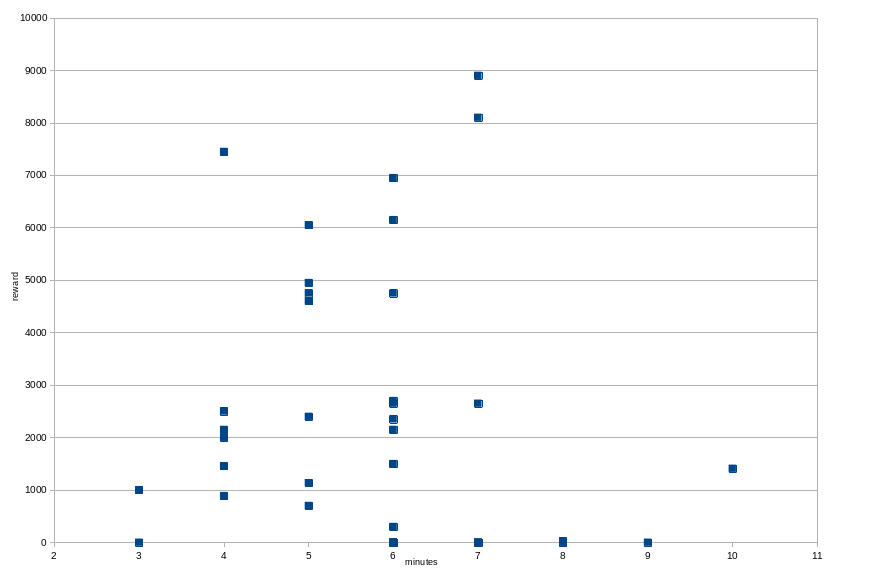
\includegraphics[width=10cm]{../time_statistics}
\end{center}
I played 253 minutes, visited 43 stations and got 92915 credits. Average duration was 5,88 minutes with standard deviation 1,47 minutes. Average reward was 2160,81 credits with standard deviation 2530,21 credits. Travel distances were between 10ly to 70ly and it seemed that all durations were totally independent from distances. I was actually playing the game so, durations include time needed to pick the best mission. Unfortunately only by writing this came to me the idea that all i had to do, so as to prove real time and game time independence during distance covering, was to record them (distance beside real duration) and calculate  correlation between them, expecting it close to 0 and away form 1. So, i did just now. I always started from Bernard's star (-1,0,0), with Xylophis equipped only with hyperdrive 1 and autopilot. I traveled without docking at intermediate stations
\begin{description}
	\item[9,63 ly] at Struve 2398 (-1,-1,1) in\textbf{ 8min} (had to travel, with 10x time acceleration, some distance across planet's surface before docking.) 
	\item[18,16 ly] at Gliese 445 (0,0,2) in\textbf{ 3min}.
	\item[24,23 ly] at Gj 1227 (-2,-1,2) in \textbf{4min}.
	\item[32,27 ly] at Deur (-1,-1,4) in \textbf{4min}.
	\item[42 ly] at  choutakyo (-1,-1,5) in \textbf{3min}.
	\item[51,94 ly] at benahamo (-1,-1,6) in \textbf{4min}.
	\item[62,97 ly] at sohiroze (0,-1,7) in \textbf{5min}.
	\item[73,75 ly] at thangria (-2,2,8) in \textbf{4min}.
	\item[84,42 ly] at ukay (-1,0,10) in \textbf{5min}.
	\item[95,71 ly] at soami (0,4,11) in \textbf{5min}.
	\item[114,06 ly] at bereshun (0,2,13) in \textbf{8min}.
\end{description}
The linear correlation coefficient is 0.307, but  even looking at distance-duration pairs make that calculation unnecessary. Average duration is 4,82min. It is less than previous 5,88min, simply because this time i did not played. I just timed pure travels.

\paragraph{The standard unit $su.$}\label{standard_unit}
\subparagraph*{One trip from station to station, without intermediate dockings or other activities than hyperjumps and traveling towards, is a standard reference unit,} when it comes to compare missions, trade activity or how well we go in game. So, let call it $ 1su $. There is no  point for a player to claim he earned 2000000 credits in 100 game years or by traveling 36000 ly. It make sense if he claims he earned 92915 credits by 43 tradings or by $ 43 su $ or he earns 2200 credits per trip or $ 2200cr/su $ or he can earn 22000 credits in 1 hour of game play.
\subparagraph{The duration of 1su} comes to unify standard and non standard activities. su is sufficient for comparing standard activities per $1 su.$ Its duration, in real minutes, is needed if we want to include in comparison non standard activities too. I assume $ 1su $ has a standard duration of 6 minutes. It seems a reasonable duration according to my recordings, i can easily remember that $ 10su $ are equivalent to 1 hour and is totally independent from player's abilities as pilot. A newbie and an expert pilot will have the same average duration of $ 1su $ per travel, concerning pure travels from station to station.
\subparagraph{The duration of 6 minutes per $1su$ is subjective} to my need of about 1 minute to decide my next in game activity. A more objective duration is that of 5 or 4,82 minutes, as i mentioned earlier.

\subsection{Non standard game activities.}

As such i mean whatever activities demand additional real time playing to complete, compared to pure trading  normal (or pure taxiing missions).  
\paragraph{A huge pro of pioneer} is that it can be seen as, or can be,  a series of normal activities, that are small duration games by themselves. If you are about to get out to visit another couple and start to get angry because you are forced to wait for your wife to complete all that female ritual you do not understand, assuming you are not part of the ritual, you can spent 6 minutes to launch from Mars, enjoy the view, be calmed by the approaching Earth and save your marriage.
\paragraph{There are two kinds of non standard activities.} Those that do not involve fighting and those that involve it. Every non standard activity has its average duration. Plus, that duration depends on player's ability of piloting. I propose the average durations of these activities to be defined accordingly to times achieved by a medium player. If game is configured on those, then experience players will get more profit per time than newbies. It does not seem unnatural.
\subparagraph*{Mining\footnote{If it exists. I tried to use pulse mining canon in several circumstances without success, nor i found some guide about it.},} and scooping its products (precious metals perhaps) would be one of them. If we call $ 1m_{u} $ the duration $ t_{mining} $ in minutes of a mining trip, from launching, mining, scooping to docking at station, then $ 1m_{u}=  \dfrac{t_{mining}}{6} su$.
\subparagraph*{Scooping and rescue missions} should have their duration units too. With same logic as above, $ 1s_{u}=\dfrac{t_{scooping}}{6} su$ and $ 1r_{u}=\dfrac{t_{rescue}}{6} su$.
\subparagraph*{Fighting} trips seems more complicated, but i think estimating an average duration of a fight mission should not be difficult for developers. My ships never was fighters and i never managed to hit my target more than once per 15minutes of fight. Luck of maneuverability because neither my crew managed to hit the target or luck of my manual abilities as pilot. It does not matter. I believe that time duration to eliminate the target or targets can be estimated, without loss of accuracy, by ECM and the number of available missiles along with their capabilities only. Assuming we defined average fight mission duration, then we similarly can have  $ 1f_{u}=\dfrac{t_{fighting}}{6} su$.
\subparagraph*{Death have the duration of $1su.$} Lets assume that the player take a fight mission. Duration from launching from station till the fight begins, plus duration from his target distraction till his next docking is still $1su.$ Lets call D the duration in $su$ of the intermediate fight itself and consider two cases. On one case, he succeeds in $1\,su+D\,su=6 minutes+6*D  minutes =t_{fighting}.$ On the other, he dies very quickly or escape or quit after fight just started and starts the same or other mission. On last case he lost only 6 minutes, or else $1su,$ without profit. For that reason, i consider that death, quit or escape actions are performed in $1su.$ 
\paragraph{The average duration of fights} for some mission can be extracted by what its author thought as fair reward for it. It is not a matter of being killed during fight or not. It is a matter of how long, excluded the needed $1su$ for travel, the fighting lasts, if player is involved in one. Lets measure the duration of fight in standard units $(su)$ and lets assume that the average fight lasts $a$ number of $su.$  That is, the average duration of mission, if a fight is to happen, equals to $(1+a)$ standard units. Let the profit of a mission be $P_{fight}.$ Lets call $Risk$ the possibility for a player, who took a mission, to be involved in some fight. A fair profit depends on the $Risk$ of the mission, so profit is a function of $Risk$, that is, profit is a function $P_{fight}(Risk).$ The player gain his profit in any case but, there is $Risk$ possibility the duration of mission to be $(1+a)\,su$ and $(1-Risk)$ possibility to be just $1su.$ The average duration would be $Risk*(a+1)+(1-Risk).$ Lets call normal profit $P_{normal}$ the profit of a mission with zero $Risk,$ that is $P_{normal}=P_{fight}(0).$ All fair profits should produce equal profits per $1su.$ So, dividing profit by the duration of mission, we get  $\dfrac{P_{fight}(Risk)}{Risk*(a+1)+(1-Risk)}=P_{normal} \Rightarrow$ 
\begin{equation}\label{eq:fight_profit}
	 P_{fight}(Risk)=P_{normal}*(1+a*Risk)
\end{equation}
where $Risk$ is the possibility for a fight to happen.
\subparagraph*{The above formula does exist in modules code,} \label{fight_duration}mostly with $a=1.$\footnote{A similar formula can be extracted for urgency. If urgency stops the player from trading alongside with the mission and trading profit is $a*Urgency$ times more than the mission's profit, then a fair profit is $Profit(Urgency)=Profit(Urgency=0)*(1+a*Urgency).$}  That does not mean that  authors of these missions instinctively agrees on that average fighting duration, from starting the attempt till destroying one target ship, is $a$ standard units. One should believe that it needs $1su$ to destroy a target ship and choses to spawn exactly one enemy ship. Other should think that there is needed $1/2su$ to destroy a ship and spawns exactly 2 enemy ships that, in total, will need $1su$ to be destroyed. A third could spawn 1 to 4 enemy ships with equal 1/4 probability assuming that each destruction needs $0.4su$ to be destroyed. All should use the same $1+1=2$ standard units as their average mission duration, but i can hardly believe that more than one could be right. If the last one is right, taking the first author's mission is easy fast money. If the first author is right, i will avoid the third's mission as too hard, slow, earned money. For now, i can do nothing about it. So, in checking the current state of the game in section \ref{currentState}, i assume all authors to be right. I assume that they control the abilities of spawned ships in a such way that affects rightfully the average fight duration of their mission.
\subparagraph*{The average duration of a mission that may include fighting} has the form of 
\begin{equation}\label{eq:fight_mission_duration}
	(1+a*Risk) \, standard\, units
\end{equation}

\section{Advertisements ignore and cancels the average reward of missions.} This is not part of a secret plan hidden in the core of the game. Just as universe do not care about the existence of earth, as earth don't care about existence of humanity, as humanity do not care about the existence of individual you, in the same way, statistics do not give a shit about our individual mission. It is the Law.
\paragraph*{Lets assume we have just created a mission that rewards a uniformly random number of credits} between A and B with $A < B$. In \textit{normal distributions} we could say that we expect average value $\mu \pm std$ meaning that 68\% of the rewards will be in $(\mu-std, \mu+std)$ interval and 95\% in $(\mu-2*std, \mu+2*std)$. Despite the fact that in our case we have uniform distribution, we can still say that we expect $\dfrac{B+A}{2}\pm\dfrac{B-A}{\sqrt{12}}$ credits, estimating that it should have the same meaning. We would be right to use the average $\dfrac{B+A}{2}$ to compute the consequences of our mission.
\subsection{Advertisements. Fast shift to maximum.} Suppose that in each station we create 3 advertisements of the same, as above, mission. The player of course, from the three advertised missions, will pick to do that with the maximum reward. Would we chose the same average value of $\dfrac{B+A}{2}$ or using the maximum B reward is a more simple and a better estimation for computing the consequences of his choices of maximum? The fast answer is that in both cases we will do the same mistake, because giving him even just 3 samples to choice, the average reward of his picks reached the $3/4$ of the $(A, B)$ interval, that is equally away from both of them.
\paragraph{The distribution of player's picks} is a \hyperref{https://en.wikipedia.org/wiki/Beta_distribution}{category}{name}{Beta distribution} and not a uniform one, every time he is able to pick the best from an advertised set of missions. The exact average of his choices of maximum from $n$ advertisements is \[ \mu=\dfrac{B*n+A}{n+1}\pm (B-A)*\sqrt{\dfrac{n}{(n+1)^2 * (n+2)}}. \]
Observe that $(n+1)^2$ is almost equal to $(n+1)^2-1$, that is \[ \dfrac{n}{(n+1)^2 * (n+2)} \approx \dfrac{n}{((n+1)^2-1) * (n+2)}=\dfrac{n}{n*(n+2) * (n+2)}=\dfrac{1}{(n+2)^2}, \] and  the whole concept is easily memorized. 
\subparagraph{The average pick of the player from $n$ advertisements}  will be the upper $\dfrac{n}{n+1}$ of mission's interval $\pm\dfrac{1}{n+2}$ of this same interval. 
\subparagraph*{The shift of average near the maximum is very fast.} If we create a mission with reward in $(0,10000)$ expecting average $5000\pm2888$, with only 4 advertisements we expect $8000\pm1633$ instead. Compared to the initial 5000, there is not much more shift left. Over double the advertisements to 9 and we expect $9000\pm905$. Give me 10000 advertisements and i will pick $9999\pm1$ on average.  
\paragraph{The number of advertisements determine both the average and the deviation of missions normalized target.} If i want to create a mission with target reward $t\pm std,$ i, primarily, have to decide the number of advertisements of that mission. Having decided that to $n,$ i can create a mission with uniformly distributed reward in $(t-n*std, t+std)$ interval, advertise it $n$ times and be accurate enough towards my goal.
\subparagraph*{It is a fact that we can arrange so, that some stations do advertise a mission more than others.} Still, we must concern only for the maximum advertised cases. The player instinctively understands that his profit is much bigger at stations where he sees a lot of advertisements than at stations where he sees only a few. Once he can not pick a satisfying mission or a commodity to trade, he will return back to a full of advertisements station or at a maximum, by trading, profit station. Even with zero profit from his comeback to 'home' trip. Do not forget that it does not matter how many stations he drifted away. The distance toward his 'home' station is always $1su.$ He will prefer the zero credits for the next $su$, if he expect to gain maximum profit for the rest ones after that.
\subsection{Mission modules, that target around same reward, affect each other.} No mission author can feel safe, even if he targeted his $t\pm std$ mission's reward in the most careful and accurate way. The advertisements of a future mission with similar target, will add to the advertisements of his mission and will shift their common average reward target farther up, perhaps getting similar to the target of a third mission and so on. Giving that, in current configuration, all ships, that can carry precious metals worthing 100000 credits\footnote{To be precise, the value must be 180000 credits because he will probably find a major export of precious metal station. In major exports it seams to be a shift to 180\% of normally available cargo.}, can be considered multi purpose ships, this fact is not neglectable. In these cases, as there is not any  mission per ship restriction, any ship(player) can carry on, any kind of mission module. In other words, all mission modules with similar target will act as one, for most types of ships(players).
\subsubsection{To avoid a mission module to act as an advertisement} of some similar target of another mission module, giving that advertisements shift up too fast towards a maximum, we must be aware, so that the maximum of our new mission's interval is in sufficient distance from the nearby maximums, of other already existed mission module targets. 
Unless of course we indeed wish to shift up an already existed average reward target, in a more elaborate way than just editing the existed target.
\subsubsection{The subjectivity of the duration of $1su$} can be seen as follows. Assume that the duration of $1su$ is $5 minutes=300seconds$ and consider a mission A of a uniformly distributed reward between (0, 10000) with exactly 4 advertisements that reveals the corresponding rewards. As described above, the average reward of this mission is easy, \[ \dfrac{4}{5}*10000=8000credits/300sec. \] Consider a new mission B, exact as mission A but with exact 5 advertisements. It could be  also easy, a better reward of $\frac{5}{6}10000=8333credits/300sec.$ However, do not reveal mission's B rewards, forcing a player to spent 3 seconds for each reward to be revealed. Now he gains 8333 credits in $300+3*5=315$ seconds, meaning \[8333/315*300=7937credits/300seconds\] a worst than mission's A reward.
\paragraph*{A player} may be satisfied by the $8000credits/300sec$ and neglect mission B. Another player may understand the benefits of advertisements and chose always to reveal all rewards of mission B, so as to have $4+5=9$ advertisements of the same target. Thus, he gains \[ \dfrac{9}{10}*10000*\dfrac{300}{315}=8571credits/300sec.\]
A third player does not want to spent time to reveal the rewards of B mission if the expected gain is less than what he has already revealed. Thus, he will not reveal the $i_{th}$ reward if he already have revealed, from missions A and B, a maximum reward greater than $\dfrac{5-i}{6-i}*10000*\dfrac{300}{300+3*(5-i)}.$ That is, he will stay on mission A if he got a reward greater than 7936 credits. He will stay on his first reveal of mission B, if the reward is greater than 7692credits. He will stay on 2nd reveal if it is greater than 7282. On 3nd if it is greater than 6536 and will reveal 5th only if the 4th reveal is lesser than 4951 credits\footnote{What is the average reward per 300 seconds of the third player's preference function, is irrelevant with my main subject and i am not willing to figure out.}.
\subparagraph*{But then,} he does not find joy in having to remember different numbers, one for each $i_{th}$ advertisement, with unrevealed reward, and asks from developers either to give him the ability to filter out the lower rewards or to reveal the rewards of advertisements all together. Developers understand that they, indirectly, are asked to reduce the maximum duration of B mission from 315 seconds to  300, so increase the rewards by 5\%\footnote{The increase happens per real time unit and not per $1su,$ because only the duration of the last is affected. Missions still complete in $1su.$}, if of course they assume that duration of revealing is 3 seconds. Generally, for the 300 seconds duration of $1su,$ the revealing of $a$ advertisements that lasts $s$ second each, will increase the rewards $\dfrac{a*s}{3}$ per cent. 300 seconds duration for $1su$ is more or less objective. What if my subjective, 360 seconds duration for $1su,$ propose is adopted? It is subjective and includes all the decision activities, of course those of revealing the rewards too. Will the 360 duration remain steady, must be reduced? What developers must do?
\subparagraph*{The concept of a standard unit} is determined well enough, i believe. Its duration, that is needed so as to be able to compare non standard activities with the standard ones, is subjective. Thanks God, i am not a developer.
\section{Current state of missions and trade.}\label{currentState} I consider it as an axiom that what motivates the in game decisions, that a player can make, is that players want to maximize their earned profit per standard unit (page \pageref{standard_unit}). Profit can be earned either by missions or by trading. Due to player's motivation, at each station he picks a mission, if mission's expected reward for the next $1su$ is greater than his profit, for the same next $1su$, by trading. Otherwise, he picks trading\footnote{Trading alongside mission in the same $su$ is rare happening and, when it happens, profit of one is much more less than the other's. So, i neglect the case of simultaneous trading during mission's trip.}. In other words, a player choses from a 2 element set of options $\{mission,trade\}.$ His preference function, that supplies an order in that set, is an easy one, it is his profit per $su$ in $credits/su$ for each element\footnote{I believe that other motivations than profit P does not exist. A killing motivation K does not include decisions making, since killing per $su$ seems constant at almost $1kill/su,$ so K seems boring, and a popularity motivation P seems at least hidden from player, such that he is unable to chase $popularity/su.$ In any case, different motivations are differnt branches of gameplay and needs their own game module analysis. In this article i care only on profit motivation P.}. 
\paragraph{Comparing states of the game} is possible only when there is an understanding of all states in comparison. Editing the configuration of the game or adding a mission module, alter the current state of the game and creates a new one. The new state alters the player's preference function, that determines his in game decisions. In order to claim that the new preference function is more interesting than the current one, we need the knowledge of the current preference function, along with that of the new state.
\subparagraph*{Current state of the game,} is something i am reference to but i luck adequate programming knowledge. So, i will describe what i see as current state of the game but i will try, along with that description, to inform about the way i got there, so as my description can be reproduced and checked by whom is interested. 
\paragraph{Simulating the missions} was the way i chosed to get my results. Comparing the maximum of intervals seems to me simple and theoretically correct but, since most, if not all, of the missions does not have constant number of advertisements but varies them from zero to some integer $n$, comparison of maximums seemed not persuasive enough.
\subparagraph*{Maxima} was the program i used for simulating. \hyperref{https://maxima.sourceforge.io/}{}{}{Maxima} is a free Computer Algebra System. As a front end of it, i used \hyperref{https://wxmaxima-developers.github.io/wxmaxima/}{}{}{wxMaxima} and his command lines will be copied in each case.  
\subsection{Mission modules.}
Generally the missions are simulated by about ten steps or commands.
\begin{enumerate}
	\item fight(x), when it exist, simulates the presence or not of enemy ships and outputs 1, meaning a fight that will last $1su$ (page \pageref{fight_duration}), or 0, meaning no fight occurred.
	\item $dstr(a)$ is the maximum reward of $a$ number of advertisements of the mission, according to my best understanding of it, reading its module code.
	\item $A[m,N]$ is a function definition that creates a sample of N elements that each is the maximum of randomly (0 to m) created advertisements.
	\item $mission:A[\#,\#]$ is the created sample list. Each element of the list is the pair $[reward, duration]$ of a sample mission.
	\item $missionReward:makelist(i[1], i, mission)$ is the list of sample rewards.
	\item $missionDuration:makelist(i[2], i, mission)$  is the list of sample corresponding  durations. 
	\item $test\_mean(mission, mean=0)$ outputs the mean value of the sample and its level of confidence.
	\item $M:mean(missionReward)$ and $D:std(missionSystemReward);$ are intermediate auxiliary values of average reward and its standard deviation, as earned, that will be used in next$\dots$
	\item $block ([L:length(mission), d:lsum(i, i, missionDuration)],$\\$    
	MeanDevPerSu:[M*L/d, D*L/d])$\\ that is the pair $[average reward, deviation]$ normalized per $1su.$ It is necessary because, when fight occurs, the duration of mission is more than $1su$. So, there is a need to divide the sum of all rewards by the the sum of durations of all the missions in the sample. 
	\item $wxhistogram(missionReward, nclasses=10)$ creates a plot of rewards, as they were earned.
\end{enumerate}
\paragraph*{For each mission, create a new file in wxMaxima} and, as his entries, copy paste the relative commands. On each one, press Shift-Enter, so as to be executed. (Or press Ctrl-Shift-R to evaluate all at once.)
\subparagraph*{Be aware that copy paste may not recognize the '\_' between 'test' and 'mean'.} In that case, insert it by hand  and press Shift-Enter. Wait few seconds and enjoy your results.
\paragraph*{I required in lua interpreter the population on Sol and few other systems.} On Sol system the output was about 16. Believing that maximum population is 16, i set the number of advertisements, accordingly to mission's module code, assuming a population of 16.
\subparagraph*{For 10000$su,$} my pc needs about 13-23 seconds. If 10000su are too much for you, alter 10000 to 1000. The results will be good enough too.
\subsubsection{Taxi.lua}
\paragraph*{UR is a list with the [urgency, risk]  pairs} of the mission\footnote{The first list, in the block we copy, defines local variables in it.}.

\begin{quote}
dstr(a):=block ([\\
\hspace*{10mm}maxim:0,dur:0,grp,i,\\
\hspace*{10mm}UR:[[0,0.001],[0,0],[0,0],\\
\hspace*{10mm}[0.13,0.73],[0.3,0.02],[0.1,0.05],[0.02,0.07],[0.15,1.0],\\
\hspace*{10mm}[0.5,0.001],[0.85,0.2],[0.9,0.4],[1.0,0.31],[0,0.17]]\\
\hspace*{10mm}],\\
for i:1 thru a do \\
\hspace*{10mm}(\\
\hspace*{10mm}Ru:1+random(length(UR)),\\
\hspace*{10mm}if $ Ru < 4$ then\\
\hspace*{20mm}(\\
\hspace*{20mm}grp:(2+random(9))/2.0*(1+UR[Ru][2])*(1+3*UR[Ru][1]),\\
\hspace*{20mm}grp:random(1.0) *3000 * grp * (0.8+random(0.4)),\\
\hspace*{20mm}if $maxim < grp$ then\\
\hspace*{30mm}(maxim: grp,\\
\hspace*{30mm}if random(1.0) $>$ UR[Ru][2] then dur:1 else dur:2\\ 
\hspace*{30mm}/*The 2 equals to 1+a, with a from (1+a*Risk)*/\\
\hspace*{30mm}  ) \\
\hspace*{20mm}else (maxim:maxim, dur:dur)\\
\hspace*{20mm})\\
\hspace*{10mm}else\\
\hspace*{20mm}(\\
\hspace*{20mm}grp:(1+UR[Ru][2])*(1+3*UR[Ru][1])/2.0,\\
\hspace*{20mm}grp:random(1.0) *3000 * grp * (0.8+random(0.4)),\\
\hspace*{20mm}if $maxim < grp$ then\\
\hspace*{30mm}(maxim: grp,\\
\hspace*{30mm}if random(1.0) $>$ UR[Ru][2] then dur:1 else dur:2 
\hspace*{20mm}) \\
\hspace*{20mm}else (maxim:maxim,dur:dur)\\
\hspace*{10mm})\\
), return([maxim,dur]))\$\\

A[m,N]:=makelist(dstr(random(m+1)), i, 1, N)\$\\
taxi:A[16,10000]\$\\
taxiReward:makelist(i[1], i, taxi)\$\\
taxiDuration:makelist(i[2], i, taxi)\$\\
test\_mean(taxiReward, mean=0);\\
M:mean(taxiReward);\\
D:std(taxiReward);\\
block ([L:length(taxi), d:lsum(i, i, taxiDuration)],  \\  
MeanDevPerSu:[M*L/d, D*L/d]);\\
Aexact[m,N]:=makelist(dstr(m), i, 1, N)\$\\
taxiExact:Aexact[16,10000]\$\\
taxiRewardExact:makelist(i[1], i, taxiExact)\$\\
test\_mean(taxiRewardExact, mean=0);\\
std(taxiRewardExact);\\
wxhistogram(taxiReward, nclasses=10);	
\end{quote}

\paragraph*{The results on my screen} are\\
MEAN TEST\\
$mean\_estimate=6212.405500448348$\\
conf\_level=0.95\\
$conf\_interval=[6143.205895789366,6281.60510510733]$\\
$std=$ 3530.054231397816\\
Normalizing per $su,$ the \textbf{taxi missions average reward is $5666\pm3219\ credits/su.$}
\subparagraph*{If the number of advertisements was constant} and you are curious about the then average, credits are outputed as taxiExact results. 
The average boosts approximately up to $8617\pm2761.$  \\*
Figure \ref{fig:taxi}, shows how many times, from 10000 stations, player got reward inside some interval.\\ 
\begin{figure}[h]
	\centering
	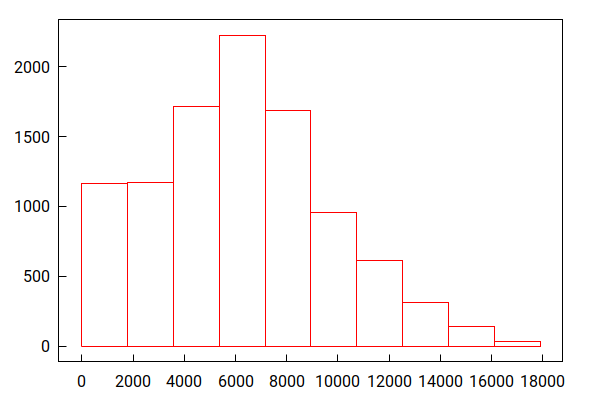
\includegraphics[width=0.8\linewidth]{../taxi}
	\caption{Taxi}
	\label{fig:taxi}
\end{figure}


\subsubsection{Assassination.lua}
\paragraph*{The procedure is the same as in module Taxi.lua.} Copy paste the below  commands\footnote{I set a=9 in this case because if maximum reputation is 16, then the module produce 0 to 16/2+1=9 advertisements.}.

\begin{quote}
	dstr(a):=block ([maxim:-1,i],\\
\hspace*{10mm}	for i:1 thru a do (\\
\hspace*{20mm}	maxim: max(maxim,\\
\hspace*{20mm}	(2100+random(4900.0) )* (1.0+random(4))\\
\hspace*{20mm}	)\\
	), return(maxim))\$\\
	
	A(m,N):=makelist(dstr(random(m+1)), i, 1, N)\$\\	
	assasin:A(9,10000)\$\\	
	test\_mean(assasin, mean=0);\\	
	std(assasin);\\
	wxhistogram(assasin, nclasses=10);
\end{quote}

\paragraph*{The results on my screen} are\\
MEAN TEST\\
$mean\_estimate16518.41466368787$\\
conf\_level=0.95\\
$conf\_interval=[16361.09144114508,16675.73788623066]$\\
$std=$ 8025.472257697836\\
 Not per $su$ because we need first to determine the duration of fights and possible fee, if player brakes the law. Don't minding about fee and considering that authors of almost all missions indirectly accept that the average duration of fight is $1su$ and in this case fight always happen, normalizing the mission could be seen as division of the results by 2. So, the \textbf{assassination missions average reward is $8259\pm4013\ credits/su.$}\\
Figure \ref{fig:assasin} shows how many times, from 10000 stations, player got reward inside some interval.\\ 
\begin{figure}[h]
	\centering
	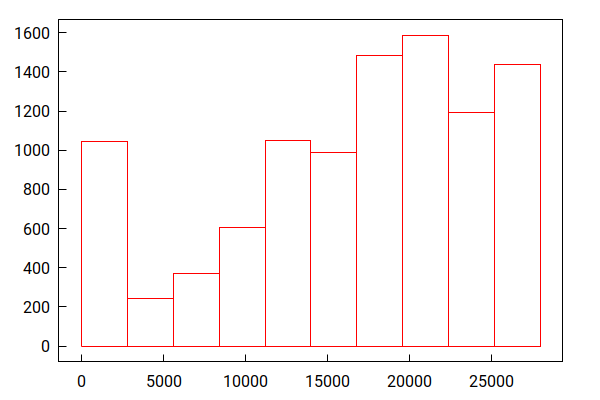
\includegraphics[width=0.8\linewidth]{../assasin}
	\caption{Assassinations}
	\label{fig:assasin}
\end{figure}
\subsubsection{CargoRun.lua - local}

\begin{quote}
dstr(a):=block ([maxim:-1,i],\\
\hspace*{10mm} for i:1 thru a do \\
\hspace*{20mm} maxim: max(maxim,\\
\hspace*{10mm}  (35+max(sqrt(random(20*1.496*100000000000))/15000,10)*\\
 \hspace*{30mm}(1.5+random(1.0))*(1+(1+random(10))/10.0))*random(2)\\
 ), return(maxim))\$\\
 
 A(m,N):=makelist(dstr(random(m+1)), i, 1, N)\$\\ 
 cargoLocal:A(16,10000)\$\\ 
 test\_mean(cargoLocal, mean=0);\\ 
 std(cargoLocal);\\ 
 wxhistogram(cargoLocal, nclasses=10)	
\end{quote}
\paragraph*{The results on my screen} are\\
MEAN TEST\\
$mean\_estimate=329.3875406512583$\\
conf\_level=0.95\\
$conf\_interval=[326.4490399623928,332.3260413401239]$\\
$std=$ 149.9006654996678\\
Normalizing per $su,$ the \textbf{local cargo run missions average reward is $329\pm150\ credits/su.$}
\begin{figure}[h]
	\centering
	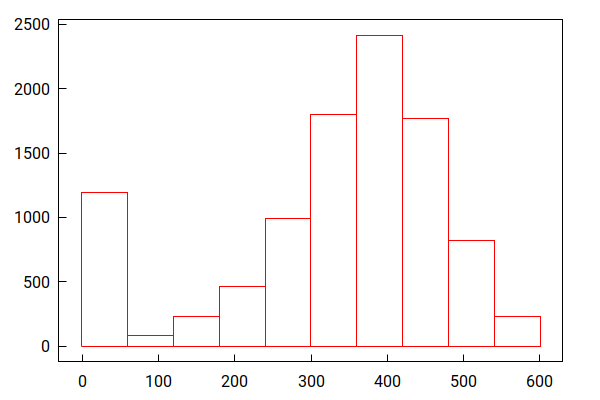
\includegraphics[width=0.8\linewidth]{../cargoLocal}
	\caption{Cargo Run local}
	\label{fig:cargolocal}
\end{figure}
\paragraph*{Because local cargo runs give different scale of rewards from the system ones,} i divided this module in two. That is the purpose of last $random(2)$ that is added at $dstr(a).$
Figure \ref{fig:cargolocal} shows how many times, from 10000 stations, player got reward inside some interval.\\ 

\subsubsection{CargoRun.lua - system}

	\begin{quote}
		
fight(x):=block(\\
\hspace*{10mm}[Risk,riskmargin,fight],\\
\hspace*{10mm}Risk:x/300.0+random(0.25),\\
\hspace*{10mm}riskmargin:0.3-random(0.6),\\
\hspace*{10mm}if (Risk $>=$ 0.5+riskmargin) then\\
\hspace*{20mm}fight:1\\
\hspace*{15mm}elseif (Risk$>=$0.2 and random(3)=0) then\\
\hspace*{20mm}fight:1\\
\hspace*{15mm}else\\
\hspace*{20mm}fight:0, return(fight)\\
\hspace*{10mm});\\		
		
	dstr(a):=block ([maxim:0,i,dur:1, reward,Rp,wholeSale,amount,\\
\hspace*{10mm}price:[50,200,20,300,10,150,50,15,20,100,10,200,200,10,250,150,\\
\hspace*{20mm}125,175,1,15,143]],\\
\hspace*{10mm}for i:1 thru a do (\\
\hspace*{20mm}wholeSale:is (random(4)=0),\\
\hspace*{30mm}if wholeSale then amount:10+random(91)\\
\hspace*{40mm} else amount:1+random(9),\\
\hspace*{50mm}Rp:1+random(length(price)),\\
\hspace*{20mm}reward: random(1.0)*(35*15)*(1+0.75*price[Rp]/300.0+random(0.25))*\\
\hspace*{30mm}(1.5+random(1.0))*(1+amount/100.0)*(0.8+random(0.4))*random(2)\\
\hspace*{40mm}/*half the times it is local cargo run,\\ 
\hspace*{50mm}that is why random(2) at the end*/,\\
\hspace*{20mm}if maxim $<$ reward then\\
\hspace*{40mm}(maxim: reward,\\
\hspace*{40mm}dur: 1+fight(price[Rp]) )\\
\hspace*{30mm}else\\
\hspace*{40mm}(maxim:maxim, dur:dur)\\
\hspace*{35mm}),\\
\hspace*{10mm}return([maxim,dur]))\$\\		
		
A[m,N]:=makelist(dstr(random(m+1)), i, 1, N)\$\\
cargoSystem:A[16,10000]\$\\
cargoSystemReward:makelist(i[1], i, cargoSystem)\$\\
cargoSystemDuration:makelist(i[2], i, cargoSystem)\$\\
test\_mean(cargoSystemReward, mean=0);\\
M:mean(cargoSystemReward);\\
D:std(cargoSystemReward);\\
block ([L:length(cargoSystem), d:lsum(i, i, cargoSystemDuration)],\\  
\hspace*{10mm}MeanDevPerSu:[M*L/d, D*L/d]);\\
wxhistogram(cargoSystemReward, nclasses=10)
\end{quote}
\paragraph*{The results on my screen} are\\
MEAN TEST\\
$mean\_estimate=1295.243834434779$\\
conf\_level=0.95\\
$conf\_interval=[1279.900280795711,1310.587388073847]$\\
$std=$ 782.7151139835458\\
Normalizing per $su,$ the \textbf{cargo run to other system missions average reward is $830\pm502\ credits/su.$}
\begin{figure}[h]
	\centering
	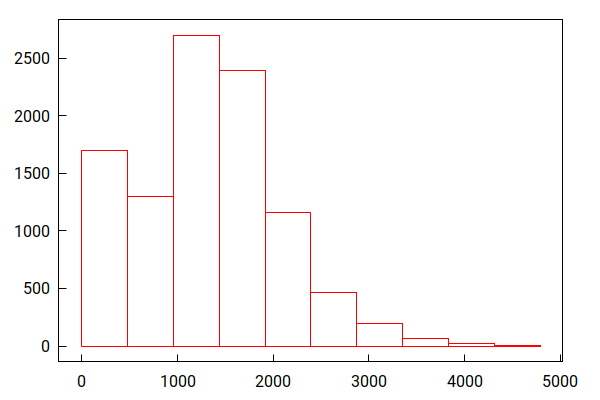
\includegraphics[width=0.8\linewidth]{../cargoSystem}
	\caption{Cargo Run to other system}
	\label{fig:cargosystem}
\end{figure}

Figure \ref{fig:cargosystem} shows how many times, from 10000 stations, player got reward inside some interval.\\ 

\subsubsection{DeliverPackage.lua}

\begin{quote}
	fight(x):=block(\\
\hspace*{10mm}	[riskmargin,fight],\\
\hspace*{20mm}	riskmargin:0.3-random(0.6),\\
\hspace*{10mm}	if (x $>=$ 0.5+riskmargin) then\\
\hspace*{20mm}	fight:1\\
\hspace*{10mm}	elseif (x $>=$0.2 and random(3)=0) then\\
\hspace*{20mm}	fight:1\\
\hspace*{10mm}	else\\
\hspace*{20mm}	fight:0,\\
\hspace*{10mm} return(fight));\\

dstr(a):=block ([maxim:0,i,reward,dur:1,\\
\hspace*{20mm}UR:[[0,0],[0.1,0],[0.6,0],[0.4,0.75],[0.1,0.1],\\
\hspace*{30mm}[0.1,0],[0.2,0],[0.4,0],[0.6,0],[0.8,0]] ],\\
\hspace*{10mm}for i:1 thru a do (\\
\hspace*{20mm}Ru:1+random(length(UR)),\\
\hspace*{20mm}if Ru $<$ 6 then\\
\hspace*{30mm}(reward:random(1.0)*(25*30)*(1+UR[Ru][2])*\\
\hspace*{40mm}(1.5+UR[Ru][1])*(0.8+random(0.4)),\\
\hspace*{30mm}if maxim $<$ reward then\\
\hspace*{40mm}(maxim: reward,\\
\hspace*{50mm}dur:1+fight(UR[Ru][2]))\\
\hspace*{30mm}else\\
\hspace*{40mm}(maxim:maxim, dur:dur)\\
\hspace*{30mm})\\
\hspace*{20mm}else\\
\hspace*{30mm}(reward:25+max(sqrt(random(20*1.496*100000000000))/15000,8)*\\
\hspace*{40mm}(1.5+UR[Ru][1]),\\
\hspace*{30mm}if maxim $<$ reward then\\
\hspace*{40mm}(maxim: reward,\\
\hspace*{40mm}dur:1+fight(UR[Ru][2]))\\
\hspace*{30mm}else\\
\hspace*{40mm}(maxim:maxim, dur:dur)\\
\hspace*{30mm})\\
\hspace*{20mm}),\\
\hspace*{10mm}return([maxim,dur]))\$\\

A[m,N]:=makelist(dstr(random(m+1)), i, 1, N)\$\\
delivery:A[16,10000]\$\\
deliveryReward:makelist(i[1], i, delivery)\$\\
deliveryDuration:makelist(i[2], i, delivery)\$\\
test\_mean(deliveryReward, mean=0);\\
M:mean(deliveryReward);\\
D:std(deliveryReward);\\
block ([L:length(delivery), d:lsum(i, i, deliveryDuration)],\\
MeanDevPerSu:[M*L/d, D*L/d]);\\
wxhistogram(deliveryReward, nclasses=10);
\end{quote}
\paragraph*{The results on my screen} are\\
MEAN TEST\\
$mean\_estimate=1180.639245062428$\\
conf\_level=0.95\\
$conf\_interval=[1167.207108132376,1194.071381992481]$\\
$std=$ 685.2087095051345\\

Normalizing per $su,$ the \textbf{delivery missions average reward is $885\pm514\ credits/su.$}
\begin{figure}[h]
	\centering
	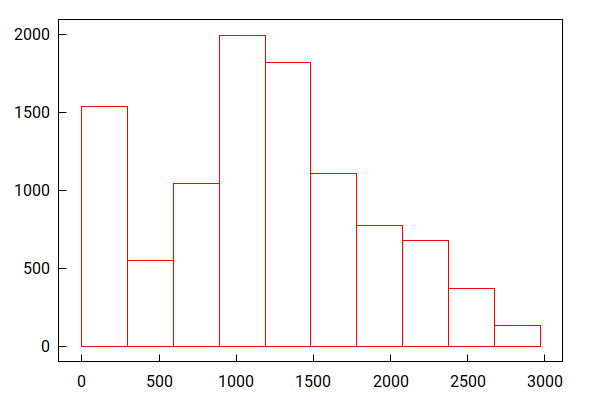
\includegraphics[width=0.8\linewidth]{../delivery}
	\caption{Delivery}
	\label{fig:delivery}
\end{figure}

Figure \ref{fig:delivery} shows how much times, from 10000 stations, player got reward inside some interval.

\subsubsection{SearchResque, Scoop and other missions} will not be touched here. They could be simulated in similar way, but they can not easily be normalized per $1su,$ because there should arise a lot of arguments about how long is their average duration. Additionally, they could be considered a different branch of game play\footnote{For example, chasing popularity or trying to rescue land,  just for fun.}, either independent from economy or, on contrary, indirectly affecting it, through qualification for missions, by raise of popularity, killings etc\footnote{To be honest, because of the major difficulty i met on rescue landing, they never attract my attention for gaining profit purposes.} So, i will save myself from the trouble of analyzing them.
\subsection{Trading} is an always present activity through which player earns credits. As such, it is simple. Buy cheap, sell expensive.
\paragraph{Prices} seems, at their normalized value, to be constant. I mean that the ratio of their increase or decrease to their defined value does not depend on the commodity itself. Unfortunately i know nothing about C language and my tries to track back the variation of prices ended at some pointers that i could not follow. So, the fluctuation of prices of commodities, as from code, remains hidden to me. I ended up to record prices of precious metals, robots, medicines and grains.
\subsubsection{Productivity modes}\label{productivityModes}
\paragraph{There are 5 productivity modes at which commodities are met on stations.} These are Major import, minor import, normal, minor export and Major export. For each commodity, on the same station, the buying price equals to the selling one. This price depends on commodity $i$, on $station$\footnote{More accurately it depends on the system where a station belongs.} and on a, by pioneer defined, function $mode(station, i)$ that outputs one of the above 5 modes.  So the price, in general, has the form of a function
 \[Price=P_{station,i}= P(station, P_{i}, mode(station,i)) \] 
 where $P_{i}$ is the nominal price of commodity $i,$ as it is defined in json files of economy module.
\paragraph{Buying and selling,} from station B to station S, is performed in $1su$ (see page \pageref{standard_unit}). Let $P_{B,i},\,P_{S,i}$ be the, corresponding to the above stations, buying and selling prices of commodity $i$ and $V_{B,i},\,V_{S,i}$ the buying and selling masses of that same commodity. Our profit equals to $P_{S,i}*V_{S,i}-P_{B,i}*V_{B,i}.$ \emph{There is no restriction on how much mass of a commodity a station can buy,} so, trying to maximize our profit per $1su,$ we are allowed to sell as much as we have bought. Because of this, we have $V_{B,i}=V_{S,i}=V^{*}_{i}.$ Then, our profit per $1su$ per $1t$  is $P_{S,i}-P_{B,i}.$
\subparagraph*{From my records it came out that prices does not depend on $station$} and have the form \begin{equation}\label{eq:price_function_P'*P}
	P_{station,i}= P'(mode(station,i))*P_{i}
\end{equation}
\label{normalized_prices} where $P'$ is a scalar function with input values the 5 modes of productivity and as output ones, just 5 numbers i needed to statistically estimate. That means that our profit per $1su$ per $1t$ \underline{per $1\,invested\,credit$} is 
\begin{equation}\label{eq:profit_per_all}
	\dfrac{P_{S,i}}{P_{B,i}}-1=\dfrac{P'(mode(S,i))}{P'(mode(B,i))}-1.
\end{equation}
 Since maximum profit from a commodity $i$\underline{ per $1credit$} of investment \emph{does not depend on its price $P_{i},$} it came to be useful to normalize my records of prices by dividing them by the nominal prices defined in json files of economy module\footnote{From normalized records, i concluded that the normalized profit of a commodity $i$ is independent from the commodity itself. So, it was not necessary to restrict my records to only 4 commodities but i could, instead of the commodity itself, to record just the productivity mode of any commodity i liked.}. Grouping my records as Major exports, minor exports, normal, minor imports and Major imports, i ended to $average\, prices \pm standard\,deviations$ of normalized prices. These were: \emph{major exports} $0.81\pm0.06,$
	\emph{minor exports} $0.93\pm0.02,$
	\emph{normal} $1.00\pm0.02,$
	\emph{minor import} $1.06\pm0.01,$
	\emph{major import} $1.17\pm0.06.$
Major modes does not have the accuracy i wished but believing that human defined average values can not deviate from a scale of 5\% without reason, I accept for average normalized prices $P'$ the following. 
\begin{description}
	\item[Major export] $P'(Major\, export)=80\%$, 
	\item[minor export]  $P'([minor\, export)=95\%$, 
	\item[normal]  $P'(normal)=100\%$, 
	\item[minor import]  $P'(minor\, import)=105\%$ and 
	\item[Major import]  $P'(Major\, import)=120\%.$
\end{description} 
I never managed to buy and sell from major to major mode. However it was easy to buy and sell from Major export to minor import or from minor export to Major import. It is expected that a player, from station B to station S, will use at least one Major mode and the best is from major export to minor import. In this case the average gain per $1su$ per investment of $1credit$ is \begin{equation}\label{eq:maximum_gain_per_1su}
	almost\,maximum\,gain\,per\,1\,credit=\dfrac{105}{80}-1=0.3125credits.
\end{equation}  His second choice offers $\dfrac{120}{95}-1=0.26credits$ per $1credit.$\\
From minor export to minor import $\dfrac{105}{95}-1=0.11credits$ per $1credit.$
\paragraph{Almost maximum gain per $1su,$} calculated as 0.3125 credits, did not take into consideration the News event module. In contrast to the trade system,  when News module is taken into consideration, profit is depended on commodity price. It has its extremes that reach up to 0.5195 credits on a low price commodity but does not alter the behavior of economy on intermediate commodities on which player does not have yet enough free cargo to buy the whole stock of the less expensive ones. This intermediate stage is the object of this article and where the almost maximum gain is referred to. I will not mention more on News module because that would make things seem more complicated than they are and would distract the attention away from the main fact that this article concerns of. That is, the economy decisions of the player is stable and do not depend on commodities he trades. So, i will keep assume the 0.3125 credits as proper value for the rest of present analysis.
\subparagraph*{If anyone wants to take into consideration the News events too,} instead of the gain of 0.3125 credits  per 1 credit on intermediate commodities, he should use the more accurate value of 0.36 credits\footnote{I assumed that, for intermediate commodities, 19 times, the profit per 1 credit, is 0.31 credit and 1 time is 2 or 3 credits but, arbitrary i accept, having available half the cargo offered by station. So, the average estimates to $(19*0.31+2.5/2)/20=0.359.$ We can not accept that we can buy full the offered cargo of News event commodity because that would mean we have one of the largest ships and we are not on the intermediate stage that this article refers to.}, after proving the rightness of this value by himself. 

\subsubsection{The normalized price $P'$ of commodities}\label{general_normalized_prices} could, in a more general form, depend on defined nominal prices too. Thus pioneer could have some, still simple, form for it, such as \begin{equation}\label{eq:general_normalized_price}
	P'(P_{i},mode(station,i))={P_{i}}^{a-1}*f(mode(station,i))
\end{equation}
 with $a$ some real number and $f$ some function from the set of modes to real numbers with $f(normal)=1$. In that case, prices would be 
\begin{equation}\label{eq:general_price}
	 P_{station,i}= f(mode(station,i))*{P_{i}}^{a}.
\end{equation}
 Assuming the players has enough cash and available free cargo, chasing the maximum profit per $1credit$ would involve trading not only  on the right mode but on the right commodity too. In current state of the game, $a=1$ so, chasing the maximum profit per $1credit$ involves only picking the right mode to trade on each station.
\subsubsection{Restrictions on trade} is a must for creating some challenge. As the per $1t$ per $1credit$ profit is given, the player maximizes his profit by maximizing his investment $P_{B,i}*V_{B,i}.$\footnote{The profit is determined by the difference between investment, as output, and earned credits from selling, as input. Restrictions on profit could be applied on both input and output terms. However, since one can sell only as much as he bought, there is no mathematical need to apply restrictions to both terms, so, i think, that defining restriction only to investment, that is to output term, is sufficient.} With no restrictions on trade, the only restriction that applies to player is his available free cargo. In that case, he picks the most expensive commodity and buys as much as his free cargo. There is no need for stock column in trade board and, at the same time, all other commodities turn to simple noise.
\paragraph{A general restriction on investment} $P_{B,i}*V_{B,i},$ but still simple with one term,  could have the form
\[
	{(P_{B,i})}^a*V_{B,i}=constant
\]
 with $a$ real number\footnote{The ${P_{B,i}}^a*{V_{B,i}}^b=constant$ may seem more general but, if $b_{th}$ root is taken on both sides then, it is clear that the result is equivalent to the in text defined restriction.}.

\subparagraph{Nominal stock $V_{i}$ is indirectly introduced in SpaceStation.lua module.}\label{nominalStock} We concern only on buying $V^{*}_{i} = V_{B,i}= V'(mode(B,i))*V_{i}.$ Player is expected to always chose $mode(B,i)=Major\_export,$ so we can write 
\begin{equation}\label{eq:nominalStock}
	V^{*}_{i}=\nu^{*}*V_{i}
\end{equation} 
with $\nu^{*}=V'(Major\_export)$ that concerns average stock. At page \pageref{averageMajorCargo} is calculated as $\nu^{*}=130\%.$  
\subparagraph*{Maximum needed cargo,} for the same mode, is
\begin{equation}\label{eq:maximumNeededCargo}
	V^{**}_i=\nu^{**}*V_{i}
\end{equation}
where $\nu^{**}=180\%,$ as calculated at the same page.
\subparagraph{General restriction} could then be written as
\[{(P_{B,i})}^a*V_{B,i}=(P'(major\_export))^{a}*P^{a}_{i}*\nu^{*}*V_{i}=constant.\]
$P^{a}_{i}$ and $V_{i}$ are the only ones that does not depend on players choice on best trade modes, so we can introduce the \emph{general restriction on trading} as
\begin{equation}\label{eq:general_invest_restriction}
	P^{a}_{i}*V_{i}=constant
\end{equation}
 
 \paragraph{Maximizing profit per $1su$} means maximizing 
 \[P_{S,i}*V_{S,i}-P_{B,i}*V_{B,i}=P_{S,i}*V^{*}_{i}-P_{B,i}*V^{*}_{i}=(P_{S,i}-P_{B,i})*V^{*}_{i}.\]
 That, using equations \eqref{eq:price_function_P'*P} and \eqref{eq:profit_per_all}, equals to
 \begin{equation}\label{eq:max_current_profit}
 	Profit_{max}= (\dfrac{P'(mode(S,i))}{P'(mode(B,i))}-1)*P'(mode(B,i))*P_{i}*\nu^{*}*V_{i}.
 \end{equation}
$V^{*}_{i}$ is restricted by the player's available cargo. So, without other restriction, player will end around a station that produce a Major mode on a commodity of the maximum $P_{i},$ the most expensive, ignoring all others.
\subparagraph*{To overcome the ignoring of all, minus one, commodities,} one can equalize all $P_{i}*V_{i}$ products of previous equation \eqref{eq:max_current_profit}, based on the fact that player can not buy more than a station can offer.
\subparagraph{Line 48 of SpaceStation.lua} does exactly this. This line of \hyperref{https://github.com/pioneerspacesim/pioneer/blob/25bc005c67a43eb2c17fcb83fe20f5d07a6b394c/data/libs/SpaceStation.lua#L48}{}{}{code} 
\begin{quote}
				local rn = 100000 / math.abs(e.price) --have about 100,000 worth of stock, per commodity
\end{quote}
is the main target of this article. \emph{It is the code expressing the general restriction of equation \eqref{eq:general_invest_restriction} with $a=1$}\footnote{Considering GetCommodityBasePriceAlterations description in Wiki, it might be, hidden in C code for me, that the percentage alteration of nominal prices depend actually on commodities. In this case one might keep logic, forms and equations from this article, but the example calculations are affected, specially the $p^{*}$, from definitions in page \pageref{sec:generalRestriction}, that mostly is taken to be equal to 0.25 for Major exports to minor imports tradings.}. By that restriction, on the assumption that a player has enough free cargo to trade some of the commodities, there is not any preference between them. All these  commodities are equal and, trading anyone of them, will fetch, at average, the same maximum profit per $1su.$ 
\subparagraph*{The assumption of enough free cargo,} however, is a weak one. When it is true in full extent the economy game is already over. Player has bought the ship with the largest available free cargo and has nothing to do with earned credits after that. On new games, the assumption is false. Player has not the available free cargo to buy even the most expensive of the commodities. Being able to buy the full stock of the most expensive commodity is his first achievement and, unfortunately, on economy point of view, almost the last one. 
 \subparagraph*{Finding a station where one can buy the whole stock of the most expensive commodity} cancels any necessity to alter, in future, to some other commodity. Thus, \emph{the general restriction with exponential $a=1$ cancels its own creation purpose}. By the current state's restriction, all commodities are equal and none will fetch more profit. When that happens, the economy branch of the game reached almost its "game over". The worst is that after finding such a station, there is not other economic motivation to get away from around that station and, if one does, there will be always the same economic motivation to run back to that station.
 \subsubsection{Trading profit per $1su$} is necessary to be estimated for comparing other activities to it. Soon enough, after a new game's start, the player will be able to buy the whole stock of the most expensive commodity, so i will start my estimation from that point.
 \paragraph{Maximum of trading profits per $1su$} happens for the first time when player gets free cargo $V^{**}_{min}$ such that he can buy the whole stock of the most expensive commodity with price $P_{max},$ on best for him modes and in accordance with the restriction of equation \eqref{eq:general_invest_restriction}. Taking this equation, with, current state's $a=1$ and considering the, more than normal, available cargo on major export mode\footnote{It is defined, in line 59 of SpaceStation.lua, as 180\% of nominal cargo.}, we get for minimum needed free cargo to get maximum trade profit \(V^{**}_{min}=\nu^{**}*V_{min}=180\%*\dfrac{constant}{P_{max}}.\) Only the 80\% is guarantied. The average of the rest (0\%-100\%) is 50\%, with standard deviation, according to code,  $\dfrac{100\%}{\sqrt{12}*\sqrt{2}}=20.41\%.$\label{MajorExportDeviation} So, the average bought cargo\label{averageMajorCargo} will be 
 \[V^{*}_{min}=(80\%+(50\%\pm20.41\%))*\dfrac{constant}{P_{max}}=(130\%\pm20.41\%)*\dfrac{constant}{P_{max}}\]\footnote{We just calculated the $\nu^{*}=130\%,$ as it was mentioned at page \pageref{nominalStock}.}.\label{std_of_v} Considering that, from equation \eqref{eq:price_function_P'*P} and Major export mode, the players buy with price $80\%*P_{max}$ per $1t,$ his average investment is $0.80*(1.30\pm0.2041)*constant=(1.04\pm0.16)*constant.$ So, from equation \eqref{eq:maximum_gain_per_1su}, we get that the average profit per $1su$ is
 \[0.3125*(1.04\pm0.16)*constant=(0.325\pm0.05)*constant\; credits\] 
 with $constant=100000,$ according to line 48 of SpaceStation.lua.
 \subparagraph{The maximum average trade profit per $1su$} is $32500\pm5000$ credits.\label{maximumCurrentTradingProfit} The reader should notice the mutual cancellation of $P_{max}$ and that, assuming there is enough free cargo, the result is the same for any price, either the maximum or the minimum or some intermediate.
 \paragraph{Minimum average profit per $1su$} could be considered zero for simplicity. The almost best pair of modes for trading, from Major export to minor import, can not happen twice in a row on same commodity. If player returns to repeat it without trading, then the second trading profit will be zero and the overall average trading profit would be half of what we just calculated as maximum, that is $16250\pm2500$ credits. However, i will not make this assumption.
 \subparagraph{The accuracy of estimation of trading profit is not important at all.} It is needed only to understand where about this profit is in relation to missions profit. \emph{The important about trading profit is that all commodities are equal and what they have to offer remains constant during the game.} In that respect, i will not hesitate to introduce a second arbitrary returning back route, after maximum profit's route, so as to avoid to use zero profit for it, since, most of times, i traded something, instead of returning with empty hands.
 \subparagraph*{The needed free cargo for maximum price commodity,} for current state of game, equals to $180\%*\dfrac{100000}{2180}=83t$\footnote{The average cargo is $130\%$ that equals to 60t, but one needs to always have 83t free cargo to achieve this.}. For second route i will assume that player trades a commodity with half the maximum price $P_{max}/2$ \footnote{Or soon after getting 80t free cargo, got double of it, 160t,  but trades a commodity that costs $P_{max}/4.$ In both cases, for maximum profit, he needs double of the cargo he has.} For returning route, he eventually finds the same pair of modes. On Major export mode, it is guaranteed to find $80\%*constant/(P_{max}/2)=160\%*constant/P_{max}$ of the $180\%*constant/(P_{max}/2)=360\%*constant/P_{max}$ cargo he needs and  he has already $180\%*constant/P_{max}$. Thus, he buys all the stock, if the value from the random 200\%\footnote{It is the interval (160\%-360\%).} is less or equal than 20\%, and restricts himself to $160\%+20\%=180\%$, if it is greater.  The average trade cargo\footnote{I calculated the average value of function $min(\dfrac{x+y}{2},0.10)$ with $x,\,y$ uniformly distributed values in (0,1), as ${\int_0}^{0.2}{\int_0}^{0.2-x}\dfrac{x+y}{2}*dx*dy+{\int_0}^{0.2}{\int^1}_{0.2-x} 0.10*dx*dy+{\int^1}_{0.2}0.10*dx.$ The standard deviation was calculated accordingly.} for this $su$ is
 \[(160\%+(19.87\%\pm1.15\%))*constant/P_{max}.\] 
 \subparagraph*{The average investment on second route} is calculated by multiplying the above cargo by $0.80*P_{max}/2,$ considering current state's $constant=100000,$
  \[
 	average\_second\_trade\_investment=71948\pm460\,credits.
 \]
\subparagraph{The average trade profit from second returning route} is found by multiplication of the above, by the profit per $1su$ of equation \eqref{eq:maximum_gain_per_1su},
\[average\_second\_trade's\_profit=22484\pm144\,credits.\]
\paragraph{Trading profit per $1su$} is found by the sum of the maximum and second route's profits divided by the duration $2su$ of both
\begin{equation}\label{eq:trade_profit}
	\dfrac{32500+22484}{2}\pm \sqrt{\dfrac{5000^2+144^2}{4}}=27492\pm2501\,credits.
\end{equation}
\subsection{Current state's overview}
\begin{figure}[h]
	\centering
	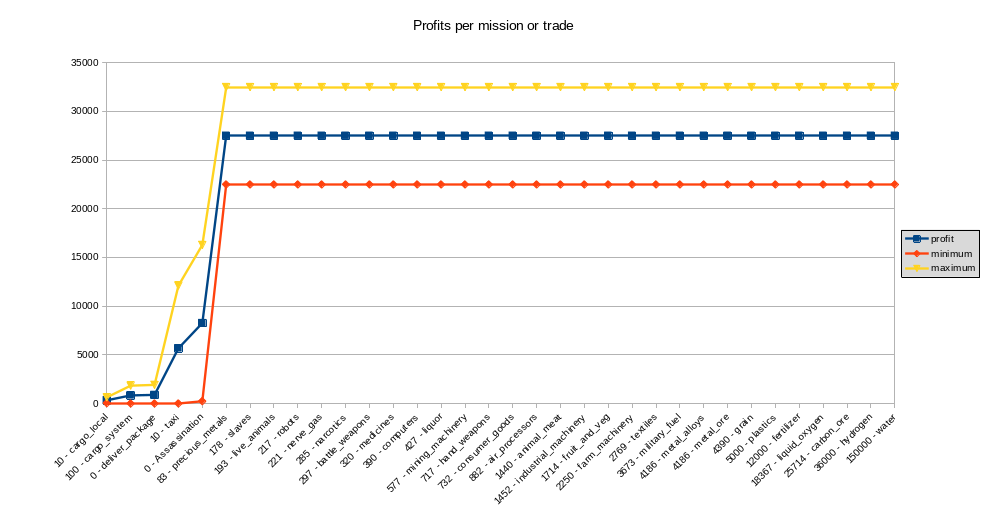
\includegraphics[width=1\linewidth]{../current_state}
	\caption{Average reward per $1su$}
	\label{fig:currentstate}
\end{figure}
Figure \ref{fig:currentstate} shows the average reward of main missions and trade. Minimums and maximums are 2 standard deviations away from the estimated average\footnote{That means that 95\% of rewards are expected to lie  between shown minimum and maximum values.}. The names on horizontal axis begin by the least free cargo needed to achieve the drawn rewards\footnote{Lines on figure are drawn for better supervision of the ascending classification. They do not represent some continuous function.}. For example, one needs at least 2769t free cargo to trade textiles or at least 83t free cargo to trade precious metals and get in both cases the 27492 credits, as average reward per $1su.$
\paragraph{Current state, on trading, is described as almost maximum.} Figure \ref{fig:currentstate} assumes that the player can buy only one commodity in its full stock of Major export mode. If he can achieve this on two commodities, his reward raises to its maximum of 32500 credits per $1su,$ instead of 27492 credits that the figure shows.
\subparagraph*{The economy branch of the game is over} for example, if he has 144000\footnote{$1.8*\dfrac{100000}{price}*0.80*price=144000$ are enough credits to buy maximum stock, on Major export mode, for the 80\% of any commodity's price.} credits, 217t\footnote{Maximum stock on Major export of robots.} free cargo and manages to find 2 stations where he buys and sells, back and forth, precious metal and robots on Major export mode. He will not target a bigger ship and different pair of commodities nor he will escape from these two stations because, even if he will not harm, definitely he will not improve his income per $1su.$  
\subsubsection{The role of missions is clearly auxiliary.}They fill the gap between start of the game till the moment player gets enough free cargo to trade the most expensive commodity. Maximum mission average profits, as only  1/3 of player's potential profit through trading or  1/5 if player avoids assassinations, is too little to influence game's economy design. After getting the ability to trade, missions does not belong to the set of player's best options, so they can not be the object of any try to alter player's behavior to a more challenging one. In current state, only trading activities can be such an object.
\paragraph{A possible course of the game in current state} could be as follows. Starting the game with nothing, lets examine figure \ref{fig:currentstate} from left to right.
\subparagraph{Delivering packages} is the only activity the player can do without free cargo and hyperdrive. This mission servers the game well, till the player gets at least his first hyperdrive, 1 passenger cabinet and yet has 1t-2t free cargo for hyperjump's hydrogen fuel in order to take, without risk, taxi missions.
\subparagraph{Taxi missions,} with five to a few tens  times more rewards than cargo-run missions, is the intermediate activity, till player gets the minimum 83t free cargo to start trading the most expensive commodity\footnote{During taxi missions, the player can keep an eye and note about systems where Major exports of precious metals happens. He will return to these systems, in order to get maximum trading profits, when he gets the minimum required free cargo of 83t for that.} on its full Major export mode extend.
\subparagraph{Trading activity} is the last activity. It will get the most profit per $1su$ in game. After finding a system B with Major export of the most expensive commodity, almost certainly a system S is found to sell and get the average of 27492 credits per $1su.$ The economy branch of the game is almost over. The only thing possibly remains\footnote{Anyway, the player does not have something better to do, from economy point of view.} is to find another Major export on system S, such that to buy and sell from and to both systems, raising the average profit per $s1u$ to its maximum of 32500 credits.
\subsubsection{Possibly rejected, from economy game play branch, activities.}
\paragraph{Assassination missions} are not part of previous possible course because of the uncertainty of their real duration. The assumption of 6 minutes\footnote{It is supposed to be the accepted duration of $1su.$} average fight duration,  described at page \ref{eq:fight_mission_duration} on section \ref{fight_duration}, is very optimistic for me. If average fight duration is longer, then the rewards are lower than those on figure \ref{fig:currentstate}. Besides that, these missions seems more appropriate to belong on different, than economy, branch of game play. I believe that they belong to a branch where player chooses to play as outlaw with the self restriction not to use trading activity. 
\paragraph{Cargo runs} are so out of economy decisions that at first i thought there should exist a wrong typo of a missing trailing zero on reward coefficients. They can serve only on the very first local station visits, alongside delivery missions, before acquisition of the very first hyperdrive. After the ability to travel onto other systems, they have almost equal to delivery missions rewards, but with the disadvantage that they require free cargo. It is a huge disadvantage. With 1t-10t free space for local runs, they are erased from the map of game decisions because of the 17 times more reward of taxi missions. With larger 10t-100t free space for system runs, they stay useless either because of taxi missions with 7 times more reward or, mainly, of the player's ability to trade (he has enough free cargo), with 33 times more reward. If a missing trailing zero was the problem, on raising their rewards tenfold, they could beat taxi missions but again, to do so, they would require such free cargo that the player already use it for trading the most expensive commodity with 3.3 times more reward. A second thought was that they served their purpose years ago and remain as a fossil of the past. But again, they are still taking work hours for maintenance. A logically natural third thought was that i miss a crucial part of the game that lead to some huge error on my estimations. I do not wish to be proven wrong, but i really do not care, as long as someone get intrigued to prove me wrong. With that feasibility interpretation, i follow with my forth thought on cargo runs mystery.
\subparagraph*{Many experienced players,} on some liked to them games, introduce self restrictions to their game play, in order to increase challenge level and maybe role playing fun. I met games that they offer challenge modes for the same purpose. A challenge mode that forbids the trading activity and taxi missions would justify the existence of cargo run missions. It make sense to let the creation of as much as possible more missions, in order to decide later on what challenge mode they belong, but the appropriate to them challenge modes are still to be developed. My opinion is that the economy branch of current state of the game is full and can not support more related to it missions. By adding more economy related missions, probably, will make economy game play worse, contrary to its most likely target to be more challenging or fun due to its challenging.
\subparagraph*{There exists the option to delete the cargo run module,} if a player wishes to. I personally chose to rename CargoRun.lua to CargoRun.lua.deleted. If a player decides to do so, before that, he must make sure that he has finished any active cargo run missions he started, otherwise he will face failure on his active missions log board. I believe that by the elimination of these module, i filtered out its missions from advertisement board and, because of this, i spent less time, by few seconds, on advertisement board on each station, raising by 1\% to 2\%\footnote{On other words, the assumption is that one spends 3.56 to 7.06 less seconds for the otherwise duration of 360 seconds of $1su.$} my rewards per real time units.
\subparagraph*{Exchange taxi and cargo system run mission's rewards} is another option that just came up to me. That is, decrease taxi rewards to the level of current cargo system run and increase the last's to the level of current taxi mission's reward. At the same time, decrease needed maximum cargo, in cargo system runs, to levels well down than 83t that are required to take full advantage of trading the most expensive commodity\footnote{Generally, decrease mission's cargo well down than that player uses for efficient trading.}, so as not to be canceled by early trading but to act as auxiliary missions till trading starts. This idea might be checked alongside with the application of general restriction on trading activity.
\section{The general restriction on trading activity.}
 As  mostly till now was the case, \emph{all trades in this section will be consider as happening from Major exports to minor imports modes}. A trading from Major to Major mode is considered just a happy coincidence. The other pairs of modes is considered a nice background noise.
\paragraph{Definitions,} that most of them used already, will help to clarify what is going on.\label{sec:generalRestriction}
\begin{description}
	\item[$P_{i}$] is the nominal price of commodity i, as it is defined in json files of economy module.
	\item[$p^{*}$] is the coefficient which, multiplied by nominal price $P_{i}$ of a commodity i, gives the profit per tone by trading that commodity. It equals to \[(\dfrac{P'(mode(S,i))}{P'(mode(B,i))}-1)*P'(mode(B,i))=P'(minor\_import)-P'(Major\_export)\] from equetion \eqref{eq:max_current_profit}.
	\item[$P^{*}_{i}$] is the profit per tone by trading commodity i. $P^{*}_{i}=p^{*}*P_{i}.$
	\item[$V_{i}$] nominal station's stock for commodity i. It is indirectly defined by nominal price $P_{i}$ and general restriction on tradining activity of equation \eqref{eq:general_invest_restriction}.
	\item[$\nu^{*}$] is the coefficient which, multiplied by nominal stock $V_{i}$ of a commodity i (see equation \eqref{eq:nominalStock}), gives the average stock on that commodity, on Major export mode.
	\item[$V^{*}_{i}$] is the average stock on commodity i, on Major export mode.  $V^{*}_{i}=\nu^{*}*V_{i}$ (see equation \eqref{eq:nominalStock}).
		\item[$\nu^{**}$] is the coefficient which, multiplied by nominal stock $V_{i}$ of a commodity i, gives the maximum possible stock on that commodity, on Major export mode (see equation \eqref{eq:maximumNeededCargo}).
	\item[$V^{**}_{i}$] is the maximum of possible station's stock on commodity i, on Major export mode. A ship must have at least that much available free cargo in order to be able to trade at average $V^{*}_{i}$ tones of commodity i. $V^{**}_{i}=\nu^{**}*V_{i}$ (see equation \eqref{eq:maximumNeededCargo}).
	\item[$P_{max}$] is the nominal price of the most expensive commodity that exists in game.
	\item[$V^{**}_{min}$] is the maximum of possible station's stock of the most expensive commodity, on Major export mode. Compared to other commodities, it is the minimum of its kind.
	\item[$V^{**}_{ship}$] is player's current   available free cargo. It must be valid that $V^{**}_{ship} >= V^{**}_{i}$ for player to be able to trade, at average, $V^{*}_{i}$ tones of commodity i. If $V^{**}_{ship} < V^{**}_{i}$, the average trading mass will be less than $V^{*}_{i}.$
	\item[$V^{**}_{maxShip}$] is the largest available free cargo, considering all the ships that exist in game\footnote{I consider $V^{**}_{maxShip}=3100t$ from Deep Space Miner and \hyperref{https://pioneerwiki.com/wiki/Category:Ships}{}{}{Wiki} where weight of hyperdrive is already subtracted from available cargo capacity. Actually it is defined as 'cargo' value in json files of ships.}.
\end{description}
\paragraph{The link between price and mass,} created only when the exponent $a$ of the general restriction \eqref{eq:general_invest_restriction} is different from 1 ($a\neq 1$), has the advantage, in contrast to the current state of the game where $a=1,$ that prices of commodities are linked uniquely to player's profits by trading them, that are linked uniquely to the available stock on these commodities, that is linked to free cargo of trading ships, that is linked to the maximum gained profit by each trading ship, that is linked to the value of each trading ship itself. This nice chain can be beneficially extended. For example, profits from trading ships can be related to profits from fightings, fightings to their duration, duration of fightings to available slots for missiles, slots for missiles to individual fighters and those must have a value, because equally valued ships is expected to gain equal profits.
\subsection{Determination of general trade restriction} can be done by the goals that developers set for game's merchant ships and the pinnacle of them. If the goal, for merchant ships, is to earn more profit by trading the most expensive commodity, in comparison from the trading  the less priced one, then smallest ships will earn faster this maximum profit than the largest ones and that, effectively, ruins the existence of large ships. So, my goal, i hope that of developers too, is to have the largest merchant ships to earn more than the smallest ones. Because of the mechanism of productivity modes (section \ref{productivityModes}) this can not be achieved by trading multiple commodities at each trip so, the goal is cheaper commodities to offer, alone, more profit from the expensive ones.
\paragraph{A relation between two commodities} can be expressed by equalizing the general restriction on them.
\[(P_{i})^{a}*V_{i}=(P_{j})^{a}*V_{j}\Rightarrow (P_{i})^{a-1}*p^{*}*P_{i}*\nu^{*}*V_{i}=(P_{j})^{a-1}*p^{*}*P_{j}*\nu^{*}*V_{j}\Rightarrow\]
\[(P_{i})^{a-1}*Profit_{i}=(P_{j})^{a-1}*Profit_{j}\Rightarrow\]
\begin{equation}\label{eq:profitRatio_ij}
	\dfrac{Profit_{j}}{Profit_{i}}=\Big(\dfrac{P_{i}}{P_{j}}\Big)^{a-1}
\end{equation}
\subparagraph*{We see, with $a>1,$ that profit from some commodity increases as its nominal price decreases.}
\paragraph{A nominal  price $P_{ship},$} with the help of the general restriction, corresponds to the $V^{**}_{ship}$ of each ship. 

\[	\left. \substack{
 	V^{**}_{ship}=\nu^{**}*{V_{ship}}\\
 	P^{a}_{ship}*V_{ship}=constant 
}\right\rbrace \Rightarrow P_{ship}=\left( \dfrac{\nu^{**}*constant}{V^{**}_{ship}}\right)^{\frac{1}{a}}
\]
Likewise, the $V^{**}_{maxShip},$ of game's crown merchant ship, corresponds to a nominal commodity minimum price
\begin{equation}\label{eq:Pship}
P_{minShip}=\left( \dfrac{\nu^{**}*constant}{V^{**}_{maxShip}}\right)^{\frac{1}{a}}.
\end{equation}

\subparagraph{The nominal $V_{min},$ corresponding to $P_{max},$} is determined by general restriction too.
\[V_{min}=constant*(P_{max})^{-a}.\]
\paragraph{Determination of general restriction} can be done by \emph{the accepted rate $R$ of trading profits increase} and by the \emph{current maximum trading profit.}
\subparagraph{Minimum nominal price} of the current largest ship is \[P_{minShip}=\dfrac{100000*\nu^{**}}{V^{**}_{maxShip}}=\dfrac{180000}{3100}=58,06\,credits.\] So, in current state, the cheapest commodity that can be effectively traded is the one that with nominal price next higher from 58.06 credits. It happens that to be 'textiles' with $P_{textiles}=65\,credits/t.$ 

\subparagraph*{Maximum profit corresponds to $P_{textile}$ that the largest ship can effectively carry.} Keeping it equal to current state's profit, by the general restriction, we decrease the profit gained from all commodities with larger nominal price and, at most, that of $P_{max}.$ New players will not be aware of that fact. However, players that already played the game, is difficult to tolerate too much reduction of the most expensive commodity. Completely subjective, i accept as less profit, gained from $P_{max},$ the $1/2.5$ of profit gained by trading 'textiles'. That corresponds $R=2.5,$ defining $R$ to be the ratio of, minimum to maximum priced commodities, profits. It is clear, since profits form all effectively traded commodities, but one, are reduced,  that \emph{the overall profit gain will be reduced}. By implementing the above, using equation \eqref{eq:profitRatio_ij}, we calculate $a.$
 \[R=\Big(\dfrac{P_{max}}{P_{textiles}}\Big)^{a-1}=\Big(\dfrac{P_{precious\_metals}}{P_{textiles}}\Big)^{a-1}\Rightarrow 2.5=\Big(\dfrac{2180}{65}\Big)^{a-1}\Rightarrow\]

	\[a=1.260851364363625.\]
We must notice that, while $a$ determines the rate by which profit varies depended on nominal prices $P_{i}$ from equation \eqref{eq:profitRatio_ij}, it also affects $P_{minShip}$ from equation \eqref{eq:Pship}. 
\subparagraph{Maximum trading profit,}  in current state, has already indirectly defined to be equal to 32500 credits per $1su$ (see page \pageref{maximumCurrentTradingProfit}) After applying the general restriction, we wish it to remain the same. So,
\begin{align*}	Profit_{textiles}=P^{*}_{textiles}*V^{*}_{textiles}=32500 \Rightarrow\\
	32500=p^{*}*P_{textiles}*\nu^{*}*constant*(P_{textiles})^{-a}\Rightarrow	
\end{align*}
\[
	constant=297098.8170256048
\]
Here, we must notice, from the above equation that, while $constant$ determines the profit  earned from trading commodity with some nominal price $P_{i},$ it also affects $P_{minShip}$ from equation \eqref{eq:Pship}.

\subparagraph*{Recapitulating,} for $\nu^{**}=1.80,$ the general trade restriction is defined by
\begin{equation}\label{results_a_for_v_1.80}
	\begin{split}
	a=1.260851364363625\\
	constant=297098.8170256048	
	\end{split}	
\end{equation}
$V^{**}_{ship},$ specially $V^{**}_{maxShip}=V^{**}_{dsminer}=3100,$ was used only to find 'textiles' as base commodity. $P_{max}$ was used only to find 'precious metals' as the most expensive commodity with $P_{max}=P_{precious\_metals}=2180.$ So, $a$ and $constant$ depend only on nominal prices of 'textiles' and 'precious metals' and, concerning $constant,$  on the wished maximum average profit too. They do not depend on $V^{**}_{ship}$ or generally on ships.
\subparagraph{Modifying Major export mode} is a serious thought i have. So, i am interesting on two other, alternatives to the above, results. So, for
$\nu^{*}=1.10,\; \nu^{**}=1.60$ and consequently $P_{minShip}=51.61,$ that is very close to nominal price 49 of 'military fuel', the results, for 'military fuel' as less priced effectively traded commodity, are
\begin{equation}\label{results_a_for_v_1.60}
	\begin{split}
		a=1.24143030154359\\ 
		constant=323774.6820117381
	\end{split}
\end{equation} and for
$\nu^{*}=1.50,\; \nu^{**}=2.00$ and $P_{minShip}=64,52,$ that points again to 'textiles' as best commodity to trade, the results, are
\begin{equation}\label{results_a_for_v_2.0}
	\begin{split}
		a=1.260851364363625.\\ 
		constant=257485.6414221913
	\end{split}
\end{equation}
\subsection{Average profit by trading commodity i.}
\paragraph{We trade commodity $i$ from station B to station S.} 
From general restriction \eqref{eq:general_invest_restriction} we get that $V_{i}=constant*P^{-a}_{i}.$ So,
\[Profit_{i}=P^{*}_{i}*V^{*}_{i}=p^{*}*P_{i}*\nu^{*}*V_{i}=p^{*}*\nu^{*}*constant*P^{1-a}_{i}.\]
$\nu^{*}$ is actually the average of a random variable, calculated as $130\%\pm20.41\%$ on page \pageref{std_of_v} and $a=1.260851364363625,$ from equation \eqref{results_a_for_v_1.80}.
Because $1-a<0,$ and clearer from equation \eqref{eq:profitRatio_ij}, we conclude that we have to trade the cheapest, possible to our ship, commodity in order to maximize our profit. But, we will have exactly the needed for that free cargo, only when $V^{**}_{ship}=V^{**}_{i}.$ 

\subparagraph*{If $V^{**}_{ship}>V^{**}_{i},$} equivalently from equation \eqref{eq:Pship} if $P_{ship}<P_{i},$ then we get lower profit than that our ship could offer, because our ship could trade more cargo on a possibly more suitable commodity. 
\subparagraph*{If $V^{**}_{ship}<V^{**}_{i},$} equivalently from equation \eqref{eq:Pship} if $P_{ship}>P_{i},$ then we get lower profit than that our ship could offer, because our ship has lower free cargo than that needed, in order to carry at average $V^{*}_{i}$ tones of commodity $i.$
\subparagraph{Players, for every ship they get, have to chose the best, from two commodities, to trade.} Those with the next higher or lower price than their $P_{ship}.$ As long as $P_{i}\neq P_{ship},$ players will get lower than their potentially maximum profit.
\subparagraph{Developers have the ability to check each commodity} so as to determine whether it can be an element of the set of commodities that players may decide to trade. Sorting nominal prices $P_{i}$ of commodities  and $P_{ship}$ of ships together, then for each commodity $i$, if the upper and lower, nearest to its nominal price $P_{i}$, values are those of other commodities, they can say that this commodity exists only as part of the noisy game's background. That because, in this case, commodity $i$ can not be part of the commodities that players may chose to trade, as there exist other commodities with nominal values closest to their $P_{ship}.$\footnote{Analogous conclusions can be extracted for ships.}
\paragraph{Each commodity can be the only one that offers, at a given moment, the potentially maximum profit.} Profit tents to increase, as available free cargo increases, in time \footnote{In contrast to current state of the game with $a=1$, where all commodities offer always the same maximum profit. With $a\neq1,$ we effectively transform the constant profit to a one to one function of commodities, whom, consequently, the inverse function exists. More accurately could exist if commodity's prices variable was some continuous interval. Since commodity prices are discrete values, the inverse function on continuous profit does not exist.}.
 \subparagraph*{In order to estimate the varying maximum profit,} i will assume that, for each commodity $i,$ there exists an ideal ship, with $P_{ship}=P_{i},$ that chose this commodity as his more efficient way to trade.
 \subsubsection{Maximum profit from station B to station S,} for an ideal ship where $P_{ship}=P_{i},$ as already expressed at the very start of this section, equals to
 \[Profit_{i}=p^{*}*\nu^{*}*P^{1-a}_{i}*constant.\]
 Equivalently, regarding the ship, using equation \eqref{eq:Pship}
  \[Profit_{shipBtoS}=p^{*}*\,\nu^{*}*\,P^{1-a}_{ship}*\,constant=p^{*}*\,\nu^{*}*\,\left( \dfrac{\nu^{**}*constant}{V^{**}_{ship}}\right)^{\frac{1-a}{a}}*\, constant.\]
  	It is the analog of 'The maximum average trade profit' paragraph at page \pageref{maximumCurrentTradingProfit}.
\subsubsection{Returning route's profit from station S to station B,} for an ideal ship trading commodity $j,$ where $P_{ship}=P_{i}$ and $P_{j}=\dfrac{P_{i}}{2},$ equals to
 \[Profit_{j}=p^{*}*P_{j}*V^{**}_{i}=p^{*}*\dfrac{P_{i}}{2}*\nu^{**}*V_{i}=p^{*}*\nu^{**}*\dfrac{P^{1-a}_{i}}{2}*constant.\]
 It is the analog of 'The average trade profit from second returning route' paragraph\footnote{Taking $V^{**}_{i}$ as the average bought stock is even more accurate than the assumption in current state. The randomness of $\nu$ happens between $(0,180\%-80\%*2^a)$ that is smaller than current state's $(0,20\%),$  as $a$ increaces away from 1.}, at page \pageref{eq:trade_profit}.
 
 Equivalently, regarding the ship, using equation \eqref{eq:Pship}
 \[Profit_{shipStoB}=p^{*}*\,\nu^{**}*\,\frac{P^{1-a}_{ship}}{2}*\,constant=p^{*}*\,\nu^{**}*\,\left( \dfrac{\nu^{**}*constant}{V^{**}_{ship}}\right)^{\frac{1-a}{a}}*\, \dfrac{constant}{2}.\]
 \subsubsection{Calculation of average profit from trading activity} is done by dividing the sum of maximum and returning profits by the duration of $2su$ of both. On all the following cases, the current state's one and the two modifications of Major export mode, the standard deviation of variable $\nu$ remains the same\footnote{Equals to 20.41\% as calculated at page \pageref{MajorExportDeviation}.}.
\paragraph{Case with $\nu^{**}=1.80$}
\[a=1.260851364363625,\;constant=297098.8170256048.\]
\subparagraph{Average profit from commodity $i.$}
\[Profit_{i}=p^{*}*\nu^{*}*P^{1-a}_{i}*constant=0.25*(1.30\pm0.2041)*P_{i}^{-0.26085}*297098.817=\cdots\]
\[(96557.11553\pm15159.46714)*P_{i}^{-0.26085}.\]
 \begin{figure}[h]
	\centering
	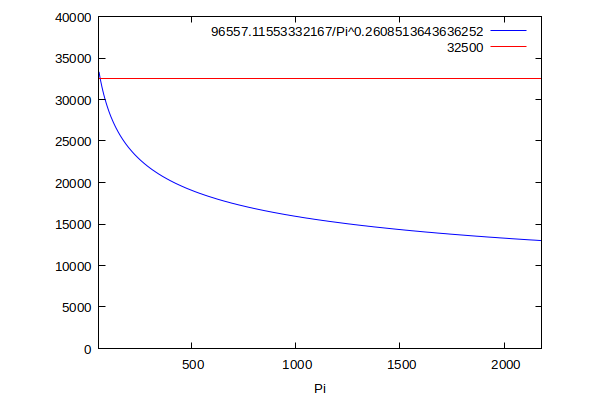
\includegraphics[width=0.8\linewidth]{../restriction_max_profit_function}
	\caption{Profile of maximum profits depended on nominal price $p_{i}$. Horizontal line is current state's maximum.}
	\label{fig:restrictionmaxprofitfunction}
\end{figure}
Figure \ref{fig:restrictionmaxprofitfunction} shows,  current state's and the applied restriction's $Profit_{i},$  profiles of maximum profits by trading, without taking into account the least profitable return route. 
 \[Profit_{j}=p^{*}*\nu^{**}*\dfrac{P^{1-a}_{i}}{2}*constant=0.25*1.80*P_{i}^{-0.26085}*297098.817/2=\cdots\]
 \[(66847.234\pm0)*P_{i}^{-0.26085}.\]
\begin{equation}\label{eq:avgProfitCommodity}
	\begin{split}
	 AverageProfit_{i}=\dfrac{Profit_{i}+Profit_{j}}{2}=\cdots\\
 (81702.175\pm7579.734)*(P_{i})^{-0.26085}
 	\end{split}
\end{equation}
\begin{figure}[h]
	\centering
	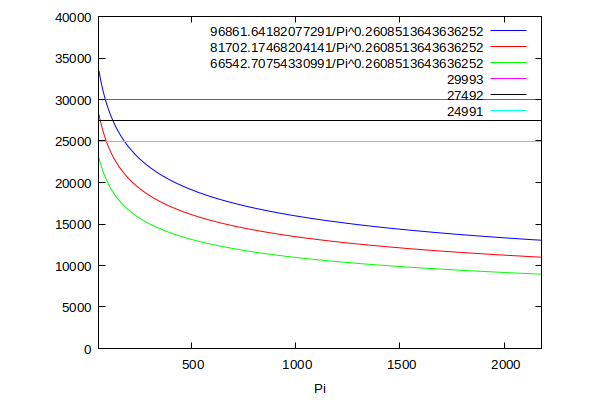
\includegraphics[width=0.8\linewidth]{../restriction_avg_profit_function}
	\caption{Profile of average profits depended on nominal price $p_{i}$. Horizontal lines is current state's average.}
	\label{fig:restrictionavgprofitfunction}
\end{figure}
 Figure \ref{fig:restrictionavgprofitfunction} shows,  current state's and the  applied restriction's $AverageProfit_{i},$ profiles of average profits by trading. Minimums and maximums are 2 standard deviations away from the estimated averages.
 
 \subparagraph{Average profit from ship.}
  \[Profit_{shipBtoS}=p^{*}*\,\nu^{*}*\,\left( \dfrac{\nu^{**}*constant}{V^{**}_{ship}}\right)^{\frac{1-a}{a}}*\, constant=\cdots\]
  \[0.25*(1.30\pm0.2041)*\left( \dfrac{1.80*297098.817}{V^{**}_{ship}}\right)^{-0.20689}*297098.817=\cdots\]
  \[(6305.37\pm989.94)*(V^{**}_{ship})^{0.20689}\]  
   \[Profit_{shipStoB}=p^{*}*\,\nu^{**}*\,\left( \dfrac{\nu^{**}*constant}{V^{**}_{ship}}\right)^{\frac{1-a}{a}}*\, \dfrac{constant}{2}=\cdots\]
    \[0.25*1.80*\,\left( \dfrac{1.80*297098.817}{V^{**}_{ship}}\right)^{-0.20689}*\, \dfrac{297098.817}{2}=\cdots\]
    \[(4365.26\pm0)*(V^{**}_{ship})^{0.20689}.\]
    \begin{equation}\label{eq:avgProfitShip}
    	\begin{split}
    AverageProfit_{ship}=\dfrac{Profit_{shipBtoS}+Profit_{shipStoB}}{2}=\cdots\\
    (5335.31\pm494.97)*(V^{**}_{ship})^{0.20689}
    	\end{split}
    \end{equation}
    
\paragraph{Case with $\nu^{**}=1.60$}\footnote{If reader downloaded the corresponding \texttt{wxmaxima} file, let replace v2:1.80 by v2:1.60 and Pc:65 by Pc:49 in first line and press Ctrl-Shift-R to reevaluate all cells.}
\[a=1.24143030154359,\;constant=323774.6820117381.\]
\[AverageProfit_{i}=(71825.53\pm7715.57)*(P_{i})^{-0.24143}\]

\paragraph{Case with $\nu^{**}=2.00$}
\[a=1.260851364363625,\;constant=257485.6414221913.\]
\[AverageProfit_{i}=(80464.26\pm6569.10)*(P_{i})^{-0.26085}\]

\subsection{General's restriction overview}
\begin{figure}[h]
	\centering
	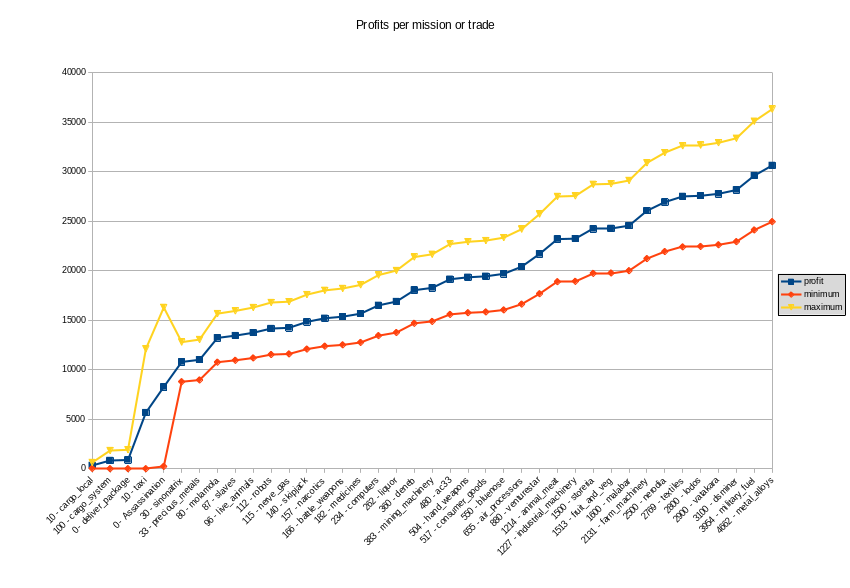
\includegraphics[width=0.9\linewidth]{../avg_restriction_state}
	\caption{General restriction's state for $R=2.5$ and $\nu^{**}=1.80.$}
	\label{fig:avgrestrictionstate}
\end{figure}
Figure \ref{fig:avgrestrictionstate} is the analog of figure \ref{fig:currentstate} on page \pageref{fig:currentstate}. It shows the average reward of main missions and trade. Minimums and maximums are 2 standard deviations away from the estimated average. The names on horizontal axis begin by the least free cargo needed to achieve the drawn rewards or by the maximum available free cargo of ships.\footnote{Lines on figure are drawn for better supervision of the ascending classification. They do not represent some continuous function.}. Ships, with the lowest $V^{**}_{ship},$ that can not effectively trade at least one commodity\footnote{Obviously,  ships with $V^{**}_{ship}<< V^{**}_{min}.$} or commodities that can not  effectively be traded by any ship\footnote{Obviously commodities $i$ with $V^{**}_{i}>>V^{**}_{maxShip}.$}, are not included in figure. That way, fighters are excluded\footnote{Fighters needs some characteristic, as free cargo is for merchant ships, that defines fighting duration and consequently their profit per $1su.$ I believe slots for missiles could be such a characteristic, but I have no simulation of some space fights  at my disposal to check it out.} from figure \ref{fig:avgrestrictionstate}.
\subsubsection{Comparing the general restriction to current state of the game} shows that there are, at least, two obvious observations.
\paragraph{Rewards from trading activities are reduced.} The left edge of horizontal, in current state, line of profits have dropped to 1/R of its initial value, thus an increasing function is created in its place. This fact may be seen as a con, but a con that coexists alongside pros, of a more challenged profit gaining and much more, as we will see.
\paragraph{Missions remain auxiliary to trading activities,} till player is able to effectively trade at least one commodity, but the transition from missions to trading activities can be designed to be smooth. Because of the happy coincidence in the choice of $R=2.5,$ we see such a smooth transition in figure \ref{fig:avgrestrictionstate}.
\subsubsection{The conversion of profit into an invertible function of nominal prices} creates a tool which gives a huge advantage in game's design in every aspect.
\paragraph{A profile of average profits, worth mentioning} and similar to that in figure \ref{fig:avgrestrictionstate}, would be the one where, on horizontal axis, $P_{i}$'s and $P_{ship}$'s alternate. In this situation, because $P_{ship}$ is ideal and probably there is not a commodity with that exact nominal price, it is difficult to say if this ship is best fitted to trade the commodity with the next, to $P_{ship}$, upper or lower $P_{i}$ value\footnote{The calculation of profit for the next upper $P_{i}$ value is already done, but the one for next lower $P_{i}$, although simple, may be proved lengthy. I am not sure but judging from the curves on figure \ref{fig:restrictionavgprofitfunction}, the best commodity to trade near high $P_{i}$s is more probable to be the one with next upper $P_{i}$ value and near low $P_{i}$s is more probable to be the one with next lower $P_{i}.$}. However, for sure, every ship is 'specialized' to trade one of them. That means, \emph{every ship is 'specialized' to trade only one commodity}. On reverse point of view, every commodity, with nominal price $P_{i},$ is best traded by one of the ships with the next, to $P_{i},$ upper or lower $P_{ship}$ value. A noisy background is probably something desirable, so there is no need to alter to such, one $P_{i}$ by one $P_{ship},$ profile. However, it is good for designers to know what is going on. With the above respect, we can see for example, in figure \ref{fig:avgrestrictionstate}, that 'computers' will not be preferred, as a commodity to trade, neither by 'skipjack' nor by 'deneb', so, more or less, 'computers' belong to the noisy background of commodities, or that 'vatakara' will not be preferred, as proper ship for trading, neither 'textiles' nor 'military fuel', so, more or less, 'vatakara' belongs to the noisy background of ships\footnote{On the assumption of course that ships classification in terms of their cost is the same as their classification in terms of their commodity 'specialization'. In any case, i can hardly believe that any ship designer dreamed for his creation to be a noisy game background. So, he may want to build a ship that specializes on a commodity that it is not already a specialization of some other ship. Of course, this possibility does not exist in current state of the game, where $a=1$.}. 
\subparagraph{Every ship is 'specialized' to trade only one commodity} and that, as a fact, reveals that there exists an invertible function between them. I introduce the symbolism $ship_{i}$ to declare that $ship$'s specialization is commodity $i.$ Thus $P_{ship_{i}}=P_{i}$ and, for $\nu^{**}=1.80,$ from equation \eqref{eq:avgProfitCommodity} 
\[ AverageProfit_{ship_{i}}=AverageProfit_{i}=
(81702.175\pm7579.734)*(P_{i})^{-0.26085}
\]
Observe that equation \eqref{eq:profitRatio_ij} remains valid.
\subsubsection{Cost value of merchant ships}
This section refers only to commodities that are the specialization of some ship. These commodities are classified by integers in such a way that \[P_{ship_{i}}=P_{i}>P_{j}=P_{ship_{j}}\] for each $i>j,$ where $i$ and $j$ are integers.
\paragraph{A game between player and salesmen} is going to be studied. The usual player tries to collect, as soon as possible, a target cash $T$ of credits, by buying or not buying merchant ships, and ship salesmen, by pricing their ships, try to sell merchant ships as expensive as they can. Player, between two ships, will prefer the cheapest one, if the expected duration, to earn his target cash, is the same on picking either of both ships. Each seller prefers to sell his ship than not to sell it, \emph{but not if that sale reduces the needed, for the player, duration,} to collect his target cash of $T$ credits, beyond some predetermined limit\footnote{This permitted but limited reduction of duration, i think, is crucial for a well defined sellers' behavior. It can be whatever developers agree on, as long seller's behavior remain stable. More on paragraph 'Ship designer's strategy' on page \pageref{designers_strategy}.}. 
\subparagraph*{There is a mathematical need for two assumptions.}
First, player and each salesman choose
the best for themselves available action, given their belief about the others’ actions. Second, everyone's belief about the others’ actions is correct. So, the normal player, knowing \emph{correctly} the guts and nuts of the game\footnote{I believe that an ambitious target of games, specially the open source ones, could be the ability to claim that they are interesting and challenging, even if they are spoiled. So, fearing to reveal the guts and nuts of some open source game can not belong to the best of attitudes.}, never makes a choice that will increase the time needed to earn his target cash and salesmen always sell their ships as expensive as they can, believing \emph{correctly} that the normal player always acts towards his best interest. 

\paragraph*{Target $T$ must exist} and can be any value. It represents the sum of costs of all things that a player would like to buy. In pioneer all costs, but those of ships, are neglectable. Characteristic choices, for $T$, are either to be equal to the largest ship's cost, where someone can assume that the economy branch of the game is over, because there is no other ship to be bought by the profit income from the largest ship, either to be equal to some tremendous large value\footnote{A choice that has the disadvantage of a tremendous increase of ships’ value because, as we will see right after, value of ships are almost proportional to the value of $T.$ A counteract, in order to avoid huge $T$, would be an introduction of some, in contrast to current state of the game, countable negative cost per $1su$. Since i did not think of that in time, in that case the whole present article would need revisit and perhaps serious alteration.}, based on the natural human greed, where player keeps wanting to earn more and more profit even if he has nothing to do with it, or, the one i prefer, some intermediate value defined perhaps by a future mission such as, for player, to earn some achievement of 'The great benefactor' of Galaxy or of some faction\footnote{Anyway, thanks to lua module mechanism, the field of 'history' or 'text' based missions, that will begin after economy branch game is over, through some great donation, or in parallel with the economy branch, is still open.}, that would be something, beyond ships, a player would like to acquire by paying its cost.
\paragraph{Lets study the 'buy-sell ship' game.} Let $B_{0}$ be the cost of player's current ship, $T$ his target cash and $B_{i}$ the cost of available ships to buy. For convenience, lets symbolize the average profit, from some $ship_{i}$ that is specialized to commodity $i$, by $q_{i}=AverageProfit_{ship_{i}}.$ 
If player decides not to buy a ship, duration needed to earn target $T$ is $d_{0}=\tfrac{T}{q_{0}}$.
If player decide to buy $ship_{i}$ with $i>0$, duration needed to earn target $T$ is $d_{i}=\tfrac{B_{i}-B_{0}/2}{q_{0}}+\tfrac{T}{q_{i}}$\footnote{All his cash was spent when he bought $ship_{i}$, so he starts to cash credits, toward his target $T$, all over again.}. Equalizing $d_{0}=d_{i}$ and solving for $B_{i}$, we find
\[B_{i}=T*(1-\dfrac{q_{0}}{q_{i}})+\dfrac{B_{0}}{2}\]
If a seller set the cost for his ship greater than the above $B_{i}$ then player will decide not to buy at all. Seller prefers to sell his ship than not to sell it, so he would like to sell it at a price just below $B_{i},$ to make it attractive for player to buy it.  For this, we can say that, for the time being, player values $ship_{i}$ at the price of $B_{i}$ credits. If $q_{i}=q_{0}$, $ship_{i}$ costs the minimum possible value of $B_{0}/2$, that equals to credits he will earn from selling his ship, so player will buy $ship_{i}$ only if it costs to him nothing. If $q_{i}\ggg q_{0}$ then the last term in parenthesis tends to zero and $B_{i}\approx T+\dfrac{B_{0}}{2}$ so, subtracting half the value of his current ship, the player will see at, bulletin board, that $ship_{i}$ costs the maximum possible value that  almost equals to his target $T.$
\subparagraph*{Same behaviour is expected from all salesmen} and player will value all ships in a similar way. All expected durations, needed for player to collect cash $T$ when he buys any ship, will be almost equal and a little less than $d_{0}\succapprox d_{i}$, so he will buy the cheapest ship. It is the one with the smallest $q_{i}$ and, because of our classification, that is $ship_{1}.$ As long as player and salesmen concern about the same and unique player's cash target, $ship_{1}$ will remain the cheapest one and that fact is independent from \emph{the correct value of $T$, that all, player and salesmen, by definition are aware of}. If, in an attempt to drop prices, player announces a much lower target $t<T$, than his real one $T$, then sellers will still keep their prices corresponding to the target  $T$. In this case too, player will prefer to buy, despite his tricky announcement, because he always prefer a duration smaller than $d_{0}$, that he will get only if he do buy. Consequently, player's real cash target is the correct value for $T$. The value of ships are the prices at which they are actually bought. So, the value of $ship_{1}$ is
\[B_{1}=T*(1-\dfrac{q_{0}}{q_{1}})+\dfrac{B_{0}}{2}\]
\subparagraph*{Just after buying $ship_{1}$,} player finds himself in the exact same situation, minus $ship_{1}$ he just bought. This time he values ships as
 \[\underset{i\neq 1}{Ship_{i}value}=T*(1-\dfrac{q_{1}}{q_{i}})+\dfrac{B_{1}}{2}\] and buys $ship_{2}$ at the price of
 \[B_{2}=T*(1-\dfrac{q_{1}}{q_{2}})+\dfrac{B_{1}}{2}\]
 The same procedure is valid till player buys the $(n-1)_{th}$, from the available at his start, ships at the price of 
 \[B_{n-1}=T*(1-\dfrac{q_{n-2}}{q_{n-1}})+\dfrac{B_{n-2}}{2}\] leaving out only the $n_{th}$, that is the game's flag ship. Advertisements for larger ship values, when current profit is $q_{current}$, equals to 
 \[\underset{i > current}{Ship_{i}value}=T*(1-\dfrac{q_{current}}{q_{i}})+\dfrac{B_{current}}{2}\]
 The above are $n-1$ equations with $B_{i}$ as $n-1$ unknowns, plus the unknown target $T$. In order to avoid to introduce, only for justifying the existence of our flag ship, some hypothetical mission's or donation's target that does not exist, i accept, as player's target, the occupation of the flag ship itself. This gives the missing $n_{th}$ equation as $Ship_{max}value-B_{n-1}/2=T$ or
 \[B_{n}=T+\dfrac{B_{n-1}}{2}\] where $B_{n}=Ship_{max}value$.
 \subparagraph*{The above forms a system of $n$ linear equations with $n$ unknows.} Developers set $B_{0}$ and $B_{n}$ values and the cost for each of the rest $n-1$ intermediate merchant ships is defined by the nominal commodity prices. Lets define, for $i=1\ldots n-1$,  $c_{i}=1-\tfrac{q_{i-1}}{q_{i}}$ and $c_{n}=1$. Then the $n$ system equations has the form
 \[B_{i}=\dfrac{B_{0}+T*\underset{k=1\ldots i}{\Sigma} 2^{k}*c_{k}}{2^{n}}\] with solution that derives by substituting
 \[T=\dfrac{2^{n}*B_{n}-B_{0}}{\underset{k=1\ldots n}{\Sigma} 2^{k}*c_{k}}
  \] to them.
 \paragraph{A static equilibrium is found.} Given that salesmen set for their ships, for $i=1\ldots n-1$, the $B_{i}$ prices,  player is not willing to alter his decision to buy all ships, one by one, and instead miss some of them, because, since the action of buying is what actually decreases duration, this would increase the needed duration to collect his target cash of $T$ credits. Sellers are not willing to alter their prices either by increasing them, because player will not buy their ship, nor by decreasing them, because they will lose credits\footnote{Unfortunately, i am a hobbyist on math field. If my knowledges would allow me the confidence of a well defined game model, i would say that the $B_{1}$ through $B_{n-1}$ prices, along with player's decision to buy with the prescribed particular order, is a \hyperref{https://en.wikipedia.org/wiki/Nash_equilibrium}{}{}{Nash equilibrium}.}. Because no one is willing to alter his action from the one that corresponds to the solution of the above system of $n$ equations, given that the actions of all others correspond to that solution, the values that are found, for the prices of $n-1$ ships, along with the decision of the player, to buy all of them, is an equilibrium. Because it will never change, it is a static equilibrium. 
 \subparagraph{Funny things} can be derived, without the need to solve the system of equations, from the 'buy-sell ship' game model and its equilibrium.
 \begin{itemize}
 	\item If authors of ship models set, for their ship, a sell price larger than its equilibrium value then their ship, mostly, will not be picked up by players. So, they put it on the game's background ships.
 	\item If authors of ship models set, for their ship, a sell price lower than its equilibrium value then they act beneficially to the player. Thus, they reduce the overall duration of the economy branch of the game.
 	\item The player's actions alone can not reduce and have him escape much from the duration of the economy branch of the game, that is expected to be a little less than $T/q_{0}$.
 \end{itemize}
\paragraph{The equilibrium's solution} was not on my initial intentions. However, i can not resist the temptation. Observation of figure \ref{fig:avgrestrictionstate} reveals that 'sinonatrix' is able to trade almost in full extend 'precious metals' or else the most expensive commodity. So, for $\nu^{**}=1.80$, \[q_{0}=Profit_{sinonatrix_{precious\_metals}}=81702.175*(P_{i})^{-0.26085}\Rightarrow\]
\[q_{0}=11000\;credits\;per\;1su\]
\[B_{0}=B_{sinonatrix}=62,707\;credits\]
and considering as the flag ship the 'Deep Space Miner' \[B_{n}=Value_{maxShip}=Value_{dsminer}=2676331\;credits\]
The 'left' or 'right' 'specialization' of each ship is roughly, by eye, estimated through figure \ref{fig:avgrestrictionstate}. Parentheses are calculated by the help of equation \eqref{eq:profitRatio_ij}\footnote{It is very tempting to use equation \eqref{eq:avgProfitShip} instead, in order to connect directly ship's free cargo and profit, but, losing ships' specialization, we lose both in accuracy and the ability to detect identical ships, when they 'specialize' to the same commodity.}. In case that more than one ships 'specialize' in the same commodity, only the cheapest one is included in equilibrium's system of equations\footnote{Including the other ships in equilibrium's system would result for them the same equilibrium value, as they trade the same commodity. So, if sellers set this as their price, the player can choose any of them without worsening his situation. For the above reason, those ships' equations can be eliminated from equilibrium's system.}. Lets write down the system of equations to solve
\begin{equation*}
	\begin{split}
	B_{1}=B_{molamola_{slaves}}=T*(1-\Big(\dfrac{P_{precious\_metals}}{P_{slaves}}\Big)^{0.26085})+\dfrac{B_{0}}{2}=0.18162*T+\dfrac{B_{0}}{2}\\
	B_{2}=B_{skipjack_{nerve\_gas}}=0.05527*T+\dfrac{B_{1}}{2}\\
	B_{3}=B_{deneb_{mining\_machinery}}=0.22106*T+\dfrac{B_{2}}{2}\\
	B_{4}=B_{ac33_{hand\_weapons}}=0.05517*T+\dfrac{B_{3}}{2}\\
	B_{5}=B_{bluenose_{consumer\_goods}}=0.00523*T+\dfrac{B_{4}}{2}\\
	B_{6}=B_{venturestar_{air\_processors}}=0.04766*T+\dfrac{B_{5}}{2}\\
	B_{7}=B_{storeria_{industrial\_machinery}}=0.12178*T+\dfrac{B_{6}}{2}\\
	B_{8}=B_{malabar_{fruit\_and\_veg}}=0.04246*T+\dfrac{B_{7}}{2}\\
	B_{9}=B_{nerodia_{farm\_machinery}}=0.06848*T+\dfrac{B_{8}}{2}\\
	B_{10}=B_{lodos_{textiles}}=0.05272*T+\dfrac{B_{9}}{2}\\
	B_{11}=B_{dsminer}=2676331=T+\dfrac{B_{10}}{2}\\
	\end{split}
\end{equation*}
Equilibrium values $B_{ship_{commodity}}$ of ships along their current prices found as\label{equilibriumSolution}
\begin{itemize}
	\item $B_{molamola_{slaves}}=490116$ with current price 81062 credits
	\item $B_{skipjack_{nerve\_gas}}=384664$  with current price 204837 credits
	\item $B_{deneb_{mining\_machinery}}=750711$  with current price 424104 credits
	\item $B_{ac33_{hand\_weapons}}=514704$  with current price 1015644 credits
	\item $B_{bluenose_{consumer\_goods}}=270575$  with current price 518244 credits
	\item $B_{venturestar_{air\_processors}}=255674$  with current price 1127263 credits	
	\item $B_{storeria_{industrial\_machinery}}=435447$  with current price 1219170 credits	
	\item $B_{malabar_{fruit\_and\_veg}}=324966$  with current price 2219852 credits
	\item $B_{nerodia_{farm\_machinery}}=335448$  with current price 2059371 credits
	\item $B_{lodos_{textiles}}=300894$  with current price 2541351 credits
	\item $T=2525884$ credits
\end{itemize}

\subparagraph{The duration of the economy branch of the game, at equilibrium prices of ships,} or more descriptively, the duration, from the moment the player gets his 'sinonatrix' till the moment he is able to buy 'Deep Space mine', is a little less than $T/q_{0}=2525884/11000=230\;standard\;units.$ If we accept the 6 minutes per $1su$, described on page \pageref{standard_unit}, the player, at equilibrium prices of ships, would need about 23 hours of game play to end the economy branch of the game\footnote{On current state of the game a rough estimation of duration, for the same target, might be $2676331/27492=97\, su$ or 9-10 hours.}.
\paragraph{The equilibrium strategy shows up.} Since player and sellers are involved in 'buy-sell ship' game, through general restriction and its 'equilibrium' consequence, a distinctive best strategy arises for both of them.
\subparagraph{Player's strategy} is a little boring\footnote{A manner of speaking. If some commodities of specializations are illegal, it remain interesting and tricky to decide between including, in the system, the respective equation as it is, including the equation after altering the specialization of the ship or omit the equation altogether.}. On exact equilibrium prices for some ship, player has no preference on any action, either to buy or not to buy this ship. Sellers or ship designers needs an advertisement to sell their ship a little cheaper. For example, 'molamola' has as equilibrium value 490116 credits. It needs an advertisement like "A molamola ship worth 490116 credits will be sold to you only for 480000, if you buy it from us". Even thus, the 'buy always' strategy seems simple enough. \emph{Player's decisions to buy or not to buy affects only themselves.} For the time being, if we apply the general restriction, but let the prices of ships intact, the equilibrium solutions prove themselves  beneficial to player. All ships, but the 'molamola', 'skipjack' and 'deneb', being too expensive, belongs to game's background and will not be sold. If we calculate the overall duration of economy branch of the game in case we buy all the ships through 'dsminer', we will need almost 38 hours of game play. So, we have to buy only the three cheapest ships. And they are very cheap, specially 'molamola'. In this case, we will need about 17 hours of game play, instead of the 23 hours, that we would need in case that prices were set by their equilibrium values. 

\subparagraph{Ship designer's strategy}\label{designers_strategy} is more interesting. With $a\ne1$, the conversion of profit into an invertible function of nominal prices, through the equation \eqref{eq:avgProfitShip}, converts profit from ship and available stock, of its 'specialized' onto commodities, into invertible functions of one to the other. As a result, it comes the equilibrium's solvable system of linear equations. Because the system is solvable, it corresponds to a restriction, between the $B_{i}$ costs of ships  and their free available cargo capacity, that converts both of them into invertible functions of one to the other too. A serious consequence is that \emph{ship designers can no longer set both the free cargo of their ship and its price.} If they set the price, they are obliged to create a ship with cargo calculated by solving one of the equilibrium's equations. If they set the cargo, they are obliged to set as price its equilibrium value. \emph{Ship designer's decisions affects almost all.} Upon adding a new ship to game, if its price equals to its equilibrium value, equilibrium prices of all ships are affected, but not the overall duration of the economy branch of the game. If its price is greater than its equilibrium value, it affects only themselves as the ship probably will not be picked up by players and belong to game's background. If its price is significantly lower than its equilibrium value, either some developer, if he wrote some 'great benefactor mission', or the designer of the game's flag ship is affected, because, by their creations, they determined the overall duration of the economy branch of the game and that is reduced because ship designer sells his ship too cheap. 
\subparagraph*{A non significant limit to the reduction of equilibrium prices,} that would act as attraction for the player to buy,  would be a fixed amount of few thousands credits, an amount about 10000 credits that will make sell price a multiple of it, a small portion, like 5\%, of the equilibrium value or something similar. Without this reduction player will not earn anything regarding his try to collect his target cash as soon as possible. He reduces duration only by the action of swapping ships. He can not buy at once another larger ship because he lacks cash. However, he can buy smaller ship gaining profit just by that action. In order to avoid that exploit, should be a disadvantage for him swapping to smaller ships. So, advertising them should be at a price greater than their equilibrium. Let $d_{current}=\tfrac{T}{q_{current}}$ the duration needed for player to collect his target cash $T$ if he does not swap ship. The duration needed if he swaps to a smaller ship is $d_{j}=\tfrac{T+B_{j}-\tfrac{B_{current}}{2}}{q_{j}}$, with $j\leq current$. Equalizing and solving for $B_{j}$ we find, for smaller, than current, ships
\[
B_{j}=T*(\dfrac{q_{j}}{q_{current}}-1)+\dfrac{B_{current}}{2}
\]
For smaller, than current, ships, advertised values could be something like
\[\underset{i \leq current}{Ship_{i}value}=5\%*T*(\dfrac{q_{i}}{q_{current}}-1)+\dfrac{B_{current}}{2}
\]\footnote{That means that maximum earned cash by swapping to smallest of ships is 5\% of $T$.}\\
For larger than current ships advertised values would be
\[\underset{i > current}{Ship_{i}value}=95\%*T*(1-\dfrac{q_{current}}{q_{i}})+\dfrac{B_{current}}{2}\] 
That means that player, in his try to collect his target $T$ 5\% faster by swapping to larger ships, succeeds exactly this and needs about 95\% of the expected duration.
\begin{figure}[h]
	\centering
	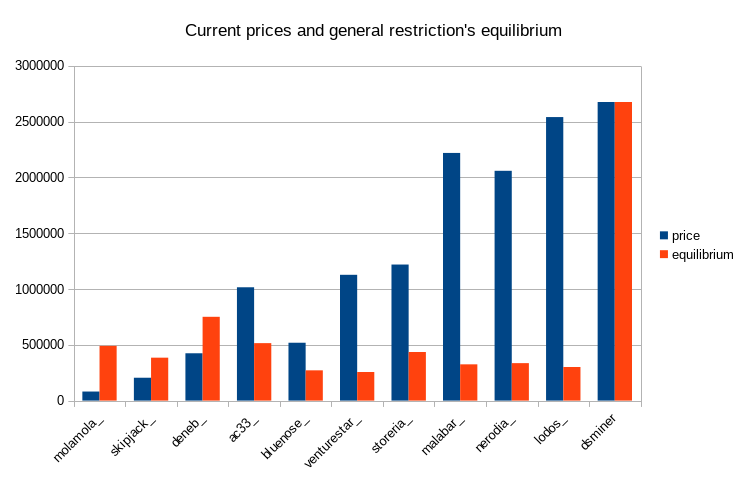
\includegraphics[width=0.9\linewidth]{../currentState_vs_equilibrium}
	\caption{Equilibrium values and current ship prices are not comparable.}
	\label{fig:currentstatevsequilibrium}
\end{figure}
\paragraph{The evolution of ship prices over time} should not escape our attention. Current ship values and the equilibrium ones, that correspond to the specific above solution, are shown on figure \ref{fig:currentstatevsequilibrium}. It is clear that equilibrium values of the prices for all medium to large merchant ships remain steadily under 500000 credits, well down from ships' current prices, and on several cases larger ships seems cheaper than smaller ones. How can it be that  the correct value, at which a large ship is actually sold, to be so small, compared to its declared value? This peculiarity happens for two reasons.
\subparagraph*{The first reason} is that equilibrium values does not capture the whole picture. They are just the sold value of a ship and not his advertised price before its sale or during the game. The nominal price of each ship, that is shown in figure \ref{fig:currentstatevsequilibrium}, as current state's of the game, is just a value. In our studied 'buy-sell ship' game model, an advertised price evolves over time, so it is an ordered set of advertised values with the selling price $B_{i}$ just the last of his elements. A value and a set of values are different things and should not be compared. That is why figure \ref{fig:currentstatevsequilibrium} might not exist, as misleading. Because all commodities offer the same profit for all ships that can effectively trade them, current state of game lacks the phenomenon of price evolution over time on ship advertisements. A phenomenon that raised naturally on our road from general restriction to the equilibrium values of selling prices. Because of this, current state includes an artificial evolution in the form that on buying a ship, from its nominal price, half the value of player's current ship is subtracted. So, cost for buying a ship artificially  evolves  over time, depending on the nominal price of our current ship. We see current state's $B_{i}$s on bulletin board as 'the cost after sell'\footnote{The creation of equilibrium's equations took into consideration the current state's artificial evolution of advertisements. This means that in the solutions run two evolutions in parallel. The artificial and the natural one. If the general restriction is to be accepted and applied, might be a good idea the removal of the artificial evolution. In this case, equilibrium's equations will take the much simpler form of $B_{i}=T*(1-\tfrac{q_{i-1}}{q_{i}})
$.}. 
\subparagraph*{The second reason} is that while in current state of the game ship designers can be considered as ship sellers, they are not the sellers of our 'buy-sell ship' game model. Ship designers do not behave accordingly to our game's model definition that wants sellers to prefer to sell their ship than not to sell it. In current state of the game, ship designers prefer not to sell in any circumstance, if player does not pay the preset price of their ship. From that perspective, the 'buy-sell ship' game is not fully present in pioneer. \emph{Player and ship designers play different games.} Player plays according to 'buy-sell ship' model observing that most station sellers are not interested to sell their ships to him, keeping them at too high prices to be useful. Ship designers play a different game, where they are not interested to sell their ships at prices near the interest of player, preferring not to sell at all and keep them on background, if they do not get the prices they want.

\subparagraph{Clarification of evolution of ship prices} may be better done by an example. Lets look at the advertisements for 'lodos' ship. While player is on hist $1_{st}$ role as 'sinonatrix', 'lodos' advertises for
\[	B_{10}=B_{lodos_{textiles}}=T*(1-\Big(\dfrac{P_{precious\_metals}}{P_{textiles}}\Big)^{0.26085})+\dfrac{B_{0}}{2}=\cdots\]
\[0.60*2525883.825+\dfrac{62707}{2}=1546884\;credits\]
 On his $2_{nd}$ role as 'molamola', 'lodos' advertisement drops to 
 \[	B_{10}=T*(1-\Big(\dfrac{P_{slaves}}{P_{textiles}}\Big)^{0.26085})+\dfrac{B_{1}}{2}=\cdots\]
 \[0.51123*2525883.825+\dfrac{490116}{2}=1536357\;credits\]
 On his $5_{th}$ role, being 'bluenose', sees
 \[	B_{10}=T*(1-\Big(\dfrac{P_{consumer\_goods}}{P_{textiles}}\Big)^{0.26085})+\dfrac{B_{5}}{2}=\cdots\]
\[0.29332*2525883.825+\dfrac{518244}{2}=1000017\;credits\]
and prices keep dropping till player as 'nerodia' buys 'lodos' for 300894 credits, that is the equilibrium solution we found for $B_{10}$.
As a fix to the peculiarity of figure \ref{fig:currentstatevsequilibrium}, ships' advertisements to 'sinonatrix' are shown on figure \ref{fig:currentstatevsequilibriumright}, where we can detect probably over priced (blue bar higher than red one) or under priced ships (blue bar lower than red one). Last ship, as common target to both states, has forcefully equally heighten bars. 
\begin{figure}[h]
	\centering
	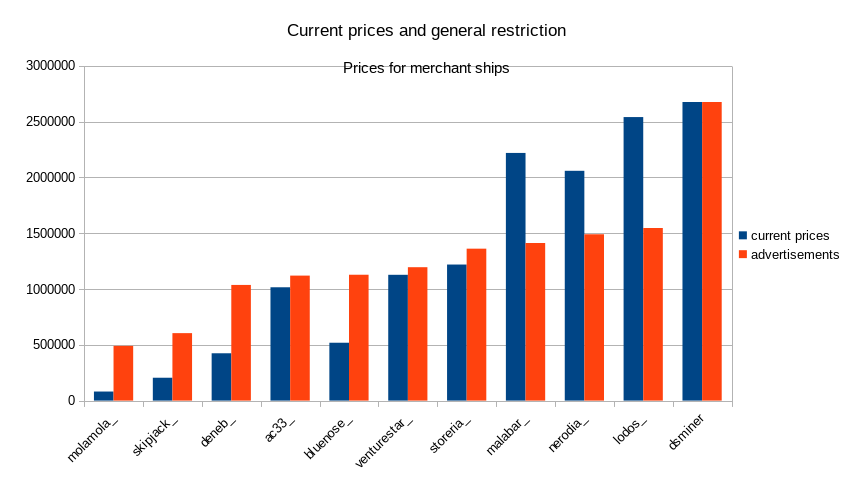
\includegraphics[width=0.9\linewidth]{../currentState_vs_equilibrium_right}
	\caption{Equilibrium's ships' advertisements toward 'sinonatrix'.}
	\label{fig:currentstatevsequilibriumright}
\end{figure}
\paragraph{The concept of ships' specialization} onto commodities adds complexity and challange to both player and ship designers. Both need to calculate which from the 'upper' or 'lower', to their ship, commodity is best to trade. Because general restriction results on invertable functions of ship profits and their free cargo from one to the other, if some ship designer wants to remove the specialization challenge from his ship, he has two possibilities.
\subparagraph*{Nearby commodity's nominal price can be adjusted.} Ship designer can set commodity's nominal price such that its $V^{**}_{i}$ to be equal to the maximum of free gargo of his ship. Take for example 'ac33' with 480t of free cargo and the nearby 'hand weapons' with $V^{**}_{hand\_weapons}=504\,t$. From equations \eqref{eq:avgProfitCommodity} and \eqref{eq:avgProfitShip} we can set
\[81702.175*(P_{i})^{-0.26085}=5335.31*(V^{**}_{ship})^{0.20689}=5335.31*480^{0.20689}\Rightarrow\]
\[P_{hand\_weapons}=261\,credits\]
instead of $P_{hand\_weapons}=251\,credits$, that is its initial nominal price.
\subparagraph*{Free cargo of ship can be adjusted.} From our example, $V^{**}_{ac33}$ can be set to 504t, instead of his initial 480t.
\subparagraph{The adjustment of the free cargo of all merchant ships} removes the specialization's challenge and, by the use of equation \eqref{eq:avgProfitShip}, the equilibrium's coefficients $c_{i}$ are easily calculated as $c_{i}=1-\big(\tfrac{V^{**}_{ship_{i-1}}}{V^{**}_{ship_{i}}}\big)^{0.20689}$, where the newly adjusted free cargos are used.

\subsubsection{Upgradable merchant ships do not fit in trading system.} 
\paragraph{The ability to upgrade merchant ships} was accepted and rejected many times in my mind so far. There are infinite upgrade mechanisms for someone to chose of. From my mind crossed finite or infinite sequences of additions or products, convergent or divergent ones. Especially after realizing the existence of the equilibrium, rejections was coming from the fact that, in order to find accurate equilibrium, every upgrade should be considered as an additional ship. Thus the number of equilibrium equations should be multiplied by the available upgrades of each ship. Even if we restrict the number of upgrades for each one ship to a small integer, together with the needed estimation of the 'specialization' of each upgraded ship, the problem was too complex to be handled accurately. The acceptances of upgrades was coming from the fact that the general restriction and the existence of equilibrium state, connect the value of a ship with its cargo. That seemed to promise a simple solution to the upgraded ships problem. Since,wiki's \hyperref{https://pioneerwiki.com/wiki/Design_Scope}{}{}{design scope} notes that \textsf{'there should be more possibilities for upgrading and customization'}, lets insist and, unfortunately, reject the idea of upgrading the merchant ships.
\paragraph{Upgrading of a merchant ship} is player's decision to increase its profit. In current state, where $a=1$, profit is constant and that, probably, makes strong the feeling that some upgrades may be needed. That is because with $a=1$ all merchant ships feels equal. In average restriction, where $a\ne1$, we have the very nice equation \eqref{eq:avgProfitShip}. It is a continuous invertable function that gives the profit of an ideal ship that always can effectively use its cargo. An upgrade on such a ship means the increase of its profit by increasing the value $V^{**}_{ship}$ or, in other words, its cargo. Assume that, at each $su$, the ship upgrades by increasing its cargo by $dV^{**}_{ship}$.  Given a minimum and a maximum cargo, the overall profit gained by a player is the integral 
\[\overset{V^{**}_{max}}{\underset{V^{**}_{min}}{\int}}5335.31*(V^{**}_{ship})^{0.20689}*dV^{**}_{ship}\]  
 The overall profit, that, if not exactly, is a major part of player's target $T$, should be and is controlled by developers at each version of pioneer, by setting minimum and maximum cargo along with the coefficient and exponential of integral's variable. These four predefined values, define the exact graph shape of the equation's \eqref{eq:avgProfitShip} profit function. Upgrades are nothing but the slopes of this graph, so the conclusion is rather clear.
 \subparagraph{Developers have already introduced all possible upgrades of merchant ships,} because, at every pioneer's version, they always set the four values that determine them. Unfortunately, slopes of profit's function does not exist because, instead of $AverageProfit_{ship}$, that is a continuous interval, in game exists only the set of discrete values $AverageProfit_{ship_{i}}$. It is not other but the set of profits of those commodities that are a 'specialization' of some merchant ship\footnote{If we keep $V^{**}_{ship}$ as a continuous interval, the profit function, being a discontinuous step forming function, does not have an invert one, that, rather loosely, i claimed as such, so often in this article. Cargo must be restricted to the set of corresponding discrete values $V^{**}_{i}$, from each 'specialized' commodity, to somehow get back the invertability, as like $AverageProfit_{ship_{i}}=AverageProfit_{ship}(V^{**}_{i})$.}. Since only the discrete values of profit exist, every upgrade means an increase from $AverageProfit_{ship_{i}}$ to $AverageProfit_{ship_{i+1}}$. For example an upgarded $deneb_{mining\_machinery}$ will be a  $deneb_{hand\_weapons}$. Its profit will be equal to $ac33_{hand\_weapons}$, so they will be ships of equal equilibrium price and we can say that the upgrade of  $deneb_{mining\_machinery}$ is the $ac33_{hand\_weapons}$, that already exist.
 \subparagraph{Upgrading is not needed} when it happens toward a commodity that is a specialization of some ship that already exists. Looking figure \ref{fig:avgrestrictionstate} can detect the 'orphan' commodities, like 'computers'. An upgrade mechanism will add unnecessary code and complexity to equilibrium equations which, hopefully, as they exist are the ones that offer to developers a simple way for firm control over the trading system.
 \subparagraph{Advertisements to ship modelers} is preferable than an upgrade mechanism, since there are not so much 'orphan', without 'specialization', commodities. For example, to cover 'computers' advertise to ship modelers that exist a need for a merchant ship with cargo $V^{**}_{computers}=234t$ (figure \ref{fig:avgrestrictionstate}). If you like the specialization's challenge for players, ask for a cargo between a near to 'computer' value, like between $V^{**}_{medicines}=182t$, and 234t. If developers like the specialization's challenge for themselves, let them find the exact $V^{**}_{ship}$ value such that 'medicines' and 'computers' will be equally preferable by the player.
\paragraph{Upgrading of merchant ships as a tool for the evolution of ship prices} is possible. If evolution of prices were to be used in game then,  for intermediate merchant ships, the one price in json ship files should be removed or not used at all and, either on the run or stored, a list of values for each ship,  one advertised price for each current ship that a player might have, should be used in their place. 
\subparagraph*{As we saw, upgrade of merchant ships is already present in game.} Lets say there was in game a merchant ship and its upgrades I, II, III, IV, V,\ldots No one would have much of objections to accept that in order to get upgrade merchant\_V one needs, as a prerequisite, merchant\_IV. Neither to set merchant\_III as a prerequisite for getting merchant\_IV and so on. Now just replace names. 'sinonatrix' for merchant\_I, 
 'molamola' for merchant\_II, 'skipjack' for merchant\_III, 'deneb' for  merchant\_IV, 
'ac33' for merchant\_V and so on, keeping the order of equilibrium solutions for $B_{ship_{i}}$ we found. All it needs a merchant ship, as additional programming code, is its prerequisite ship, if there is defined one by equilibrium equations, and, as a fix to its price, a replacement of the price value in its json file, with the corresponding $B_{ship_{i}}$ equilibrium solution.\label{prerequisiteShips}
\subparagraph{Evolution of prices and merchant ships upgrade together,} are, by this way, successfully camouflaged behind the prerequisite ships, without the need for additional elaborate programming code, but, for the knowledgeable, only a trivial one.
\subparagraph*{What we gain is} that, instead of stopping on the third ship 'deneb' and its 'mining machinery' specialization, towards our struggle to get 'dsminer', we keep trying searching our fortune to seven more ships, commodities and systems.
\subparagraph{Another option of upgrades,} if prerequisite is to be accepted, is a series of ships, for example 'lodos-I'\ldots'lodos-X' or 'vatakara-I'\ldots'vatakara-X' etc, that will have prerequisites of their kind and that all will be of about equal cargo and prices beginning with cargo $V^{**}_{1}$ and price $B_{1}$ and ending with cargo $V^{**}_{10}$ and price $B_{10}$. That way the same avatar ship will be kept.

\section{Comparison between states}
Lets try to imaginary play both states, current and general restriction applied, so as to detect similarities and differences in their game play.
\paragraph*{On both states} player starts with missions.
\subparagraph*{On current state,} the transition, from missions to fully extended traded activities, is steep.
\subparagraph*{On general restriction,} because the profit from the most expensive commodity is lowered, the transition is smoothed.
\paragraph{On both states} player moves around a station that stocks the most profitable to him commodity.
\subparagraph*{On current state,} player moves around only one station that major exports the most valuable commodity. As soon as he gets a rather small ship that can trade the full stock of that commodity, there is \emph{never} any economical benefit to get away from that station, to buy a larger ship or alter trading commodity, for the rest of the game. The economy branch of the game is over too soon, well before player reaches his probable economy target to collect a certain amount of cash. This fact seems consistent with the \hyperref{https://pioneerwiki.com/wiki/Design_Scope}{}{}{design scope} of the game, where is noted \textsf{'Your hard-earned spaceship is your avatar, and also your home. A player should become attached to it. Spaceships should be very expensive to own and maintain.'}
\subparagraph*{On general restriction,} player moves around one different station per acquired ship. It is beneficial for the player to \emph{always} alter to a cheaper commodity and, consequently, to both find another station, that major exports it, and get a larger ship. The economy branch of the game do not end, till player reaches his probable economy target to collect a certain amount of cash. This fact seems in contrast to design scope of the game. It is like an alteration to a scope that says \emph{'Changing avatar should not give significant advantage. The expected duration of economy branch of the game should remain stable and firmly controlled'}.   
\paragraph{On both states} chase for better profit per $1su$ stops soon, one or two ships after 'sinonatrix'.
\subparagraph*{On current state,} the short, 'one or two ships', ending of interest for better profit can not be avoided.
\subparagraph*{On general restriction,} interest for better profit can last up to ten ships, if we fix ship prices and add a prerequisite ship where our equilibrium solutions demonstrate the need for its existence. 

\label{pages_for_48_lua_line}
\section{Request for creation of simple Pull Requests}

\subsection{A simple Pull Request (first version).}
I wrote \getpagerefnumber{pages_for_48_lua_line} pages in this article because i was unable to find a short, five lined and convincing the right people, comment, accompanying a Pull Request, concerning the change just of the $48_{th}$ line of \hyperref{https://github.com/pioneerspacesim/pioneer/blob/25bc005c67a43eb2c17fcb83fe20f5d07a6b394c/data/libs/SpaceStation.lua#L48}{}{}{SpaceStation.lua}.
\paragraph{My propose for a Pull Request} is to change this line from
\begin{quote}
	local rn = 100000 / math.abs(e.price)
\end{quote}
into what the application of the general restriction suggest, by equation \eqref{results_a_for_v_1.80} in page \pageref{results_a_for_v_1.80},
\begin{quote}
	local rn = 297098.8170256048 / math.abs(e.price)\textasciicircum1.260851364363625\footnote{In case that a general restriction on profit is already present in C code, the equation \eqref{eq:general_invest_restriction} takes the form \[V_{i}=\dfrac{constant}{P^{a}_{i}}=\dfrac{constant}{P^{*}_{i}/(f(Major\_export)-f(minor\_import))}\Rightarrow\]\[V_{i}=\dfrac{constant}{P^{*}_{i}}*(f(Major\_export)-f(minor\_import))\] where $f(mode)$ is that of equation \eqref{eq:general_price}. In this case, i suppose that $e.price$ of lua line equals to $P^{*}_{i}$ and should not set additional exponential to it. It should be better to fix $a$ in C code and correct the result for $constant$ multiplying it by the difference of the above $f(mode)$s.}
\end{quote}

I do not know if my decision, to replace a five line comment\footnote{as it was appropriate to do for an one line concerned PR} by a \getpagerefnumber{pages_for_48_lua_line}\textminus page article, will be proved useful to anyone, but in those pages are covered many aspects of game's trading economy. All \getpagerefnumber{pages_for_48_lua_line} pages and all their covered aspects have to do with the implementation of the general restriction, by alteration of that one $48_{th}$ line. \textbf{\textsl{One line to rule them all, one line to find them, one line to bring them all and, in the game's trading system, bind them.}}
\subparagraph*{This change alone can not offer its full potential} and much of change to the current state of the game, except that it makes trading a little harder. Fixing of ship prices at their respective json files in "data/ships" folder is needed, replacing them by the equilibrium's solution in page \pageref{equilibriumSolution}, reduced a little, as described on paragraph 'Ship designer's strategy' on page \pageref{designers_strategy}. The above is easy for anyone and does not envolve compilation of the game either. Of course, since i am not able to write the necessary, for prerequisite ships, code, that was mentioned on page \pageref{prerequisiteShips}, \emph{one has to restrict himself to acquire ships only in the order of equilibrium's solution}\footnote{It is not right, either joyful, to buy, for example, 'lodos' for 300894 credits, just because i am unable to write code that will not allow me to do so, unless i sell 'nerodia'. A record on custom log of bulletin board can act as an in game reminder of the acquiring ships order.}.
\subparagraph*{A game's bulletin board advise} of the form \textsf{"Low priced commodities can offer more profit, but they need sufficient ship cargo space to do so."} might point to the general restriction's implementation.
\subsection{Extending the simple Pull Request (second version).}
Player, in his try to collect a cash target as soon as possible, stays, in current state of game, around a system that major exports the most precious commodity. If we apply general restriction in its full extend, player stays around ten such systems, one for each of his ships, that major exports the commodity on which each of his ships is 'specialized'. 
\paragraph{An attempt to lure player to explore,} more than ten systems, is to increase his profit when he visits a system for his first time. Because Major export is the most used mode, there is no real need to alter other modes too. An advise of the form "In an attempt to lure you as costumer, station sellers major exports to you more stock when you first visit their system." could point player to the benefits of exploring.
\paragraph{My propose for Pull Request's extention} is to change $59_{th}$ line,  of the same \hyperref{https://github.com/pioneerspacesim/pioneer/blob/25bc005c67a43eb2c17fcb83fe20f5d07a6b394c/data/libs/SpaceStation.lua#L59}{}{}{SpaceStation.lua}, file from
\begin{quote}
	stock = stock + (rn*0.8)
\end{quote}
to
\begin{quote}
	stock = stock + (Game.system.explored and (rn*0.6) or (rn))
\end{quote}
\emph{I have not tested yet this propose.} May be it is not too attractive the benefit to apply just once per explored system and every time to look out for a new system, just after you found one you like, according to your specialization. May be it would be preferable the more major export period to last, lets say, 6 months from the moment you first visited a system. May be it takes too much time seeking far away systems that Major export your specialization. That would increase the real time duration of $1su$ and could cancel the benefit. Anyway, the idea seems to me attractive and easily applied. That is why i mention this second propose and why i calculated $a$ and $constant$ for this occasion, just after equation \eqref{eq:avgProfitShip}, even if used these results nowhere. 

\subsection{Tickling the missions}
Missions are found as offering less profit than trading actions and that is why they can be characterized as auxiliary to trading. Observe figure \ref{fig:currentstate}. One can say that 'taxi' missions earn the $1/5_{th}$ of trading profit, but is ambiguous to tell if this ratio is about small or large ships, because all ships offer the same profit. With general restriction applied, this ambiguity is over. Observe figure \ref{fig:avgrestrictionstate}. This time one can tell that 'taxi' missions earn the same ratio $1/5_{th}$ of maximum trading profit or $1/2_{th}$ of minimum trading profit and they act auxiliary exactly for this minimum, till player starts earning this through trading. Minimum and maximum trading profits are static. If we see missions as a ratio of them, we need to do nothing. However, if we see them as a safe zone for the lowest profit, at times where player is not yet capable to trade effectively, why not to see them to act as a safe zone all the time? Why not to offer  $1/2_{th}$ of player's trading profit all the time? In that case, we can connect mission rewards with player's trading profit with the help of equation \eqref{eq:avgProfitShip}. We would like their reward to be either the current one or $1/2_{th}$ of player's current trading profit, if it is greater. Since i have trouble to get even my current ship's available cargo space, i will use pseudo code for my final propose. 
\paragraph{My propose for mission's tickling,} through  pseudo code, is to alter typical rewards in lua missions' files to
\[
	new typical reward = max(typical reward, \dfrac{typical reward}{11000}*5335.31*(V^{**}_{ship})^{0.20689})
\]
where 11000 is the minimum efficient trading reward from 'sinonatrix' and the rest is equation \eqref{eq:avgProfitShip} that gives the ideal reward of a ship without 'specialization'. This way, missions will have rewards with stable ratio to trading profits, that equals to the ratio that they currently have with minimum trading profits.
\section*{This is the end}
I do not claim that my calculations are right. I leave this responsibility to whom will be intrigued to accept them as right. The main idea behind this article is that a clarified game model, that governs player's decisions, can help contributors to be in "path" and their creations to coexist in harmony.\\
\emph{I wish the best for our game.}\\
I thank you very much my reader friend, since you made it this far.
\begin{center}
	"The End"\\
	\vspace{5mm}	
	This is the end\\
	Beautiful friend\\
	This is the end\\
	My only friend\\
	
	The end\\
	Of our elaborate plans\\
	The end\\
	Of everything that stands\\
	The end\\
	No safety or surprise\\
	The end
	\begin{flushright}
		Doors
	\end{flushright}
\end{center}

\end{document}
